
%% Preâmbulo (configurações, pacotes e tudo mais)
\documentclass[
	article,			% Define que este será um artigo (e não uma tese/monografia/relatório)
	12pt,				% Fonte: 12pt
	oneside,			% Impressão: oneside = 1 face, twoside = 2 faces (frente-e-verso)
    %openright,			% capítulos começam em página ímpar (use apenas se usar "twoside")
	a4paper,			% Tamanho do Papel: A4
    chapter=TITLE,		% Todos os capítulos devem ficam em caixa alta
    section=TITLE,		% Todas as seções devem ficar em caixa alta
	%english,			% Adiciona Idioma para Hifenização: Inglês
    %spanish,			% Adiciona Idioma para Hifenização: Espanhol
    %french,			% Adiciona Idioma para Hifenização: Francês
	brazil				% Adiciona Idioma para Hifenização: Português do Brasil (o último idioma se torna o principal do documento)
]{abntex2}				% Utilizar ABNTeX2

%% Preambulo LaTeX 
%% Definições do documento

%% Tipografia
%% Abra este arquivo e selecione uma das opções de fonte nele. A padrão é Times.
%% Tipografia / Fontes
%% AVISO: Todas essas fontes são *bastante semelhantes* aos nomes com as quais as descrevo. Entenda: são iguais, só que oficialmente com outro nome.

%% %%%%%%%%%%%%%%%%%%%%%%%%%%%%%%%%%%%%%%%%%%%%%%%%%%%%% %%
%% Comente todas as outras fontes que você não vai usar! %%
%% %%%%%%%%%%%%%%%%%%%%%%%%%%%%%%%%%%%%%%%%%%%%%%%%%%%%% %%

%% Latin Modern (fonte padrão do LaTeX, Computer Modern, mas com suporte a caracteres acentuados)
%% Considerada a mais clássica e bonita
%\usepackage{lmodern}



%% Times
%% Considerada a mais confortável de ler quando impresso
%%\usepackage{mathptmx}

%% Variação da mesma fonte, com minúsculas diferenças entre uma e outra (coisas bastante técnicas como kerning, aliasing e afins) - Essa tem revisões frequentes
%\usepackage{newtxtext} \usepackage{newtxmath}



%% Arial
%% Considerada mais confortável de ler num computador
%% ** Oficialmente recomendada pelo manual de formatação do IFPI **
\usepackage{helvet} \renewcommand{\familydefault}{\sfdefault}



%% Palatino
%% Uma opção mais elegante à Times
%\usepackage{newpxtext}



%% Kepler
%% Variação evoluída da Palatino, com várias pequenas diferenças e refinamentos
%\usepackage{kpfonts}

%% Libertine
%% Uma fonte estilo Serif comum no Linux
%\usepackage{libertine} %\usepackage[libertine]{newtxmath}

%% Estilização de Headings [ Capítulo, Seção, Subseção, Subsubseção ]

\usepackage{titlesec}                   % Pacote para formatação de títulos

\titleformat{\chapter}
{\normalfont\normalsize\bfseries\MakeUppercase}{\thechapter}{1em}{\vspace{1em}}{}
\titleformat{\section}
  {\normalfont\normalsize\MakeUppercase}{\thesection.}{1em}{}
\titleformat{\subsection}
  {\normalfont\normalsize\bfseries}{\thesubsection.}{1em}{}
\titleformat{\subsubsection}
  {\normalfont\normalsize\itshape}{\thesubsubsection.}{1em}{}

\counterwithin{section}{chapter}

\titlespacing{\chapter}{0pt}{0pt}{0pt}



\usepackage[T1]{fontenc}				% Seleção de códigos de fonte.
\usepackage[utf8]{inputenc}				% Codificação do documento (conversão automática dos acentos)
\usepackage{indentfirst}				% Indenta o primeiro parágrafo de cada seção.
\usepackage{nomencl} 					% Usado pela Lista de símbolos
\usepackage{color}						% Controle das cores
\usepackage{graphicx}					% Inclusão de gráficos
\usepackage{float}						% Melhorias para posicionamento de gráficos e tabelas
\usepackage{microtype} 					% Melhorias na justificação
\usepackage{lastpage}   		        % Dá acesso ao número da última página do documento
\usepackage{booktabs}					% Comandos para tabelas
\usepackage{multirow, array}			% Múltiplas linhas e colunas em tabelas
\usepackage{longtable}					% Tabelas que quebram entre páginas

\usepackage[table,xcdraw, dvipsnames]{xcolor}       % Cores para tabelas e elementos textuais
\usepackage[brazilian,hyperpageref]{backref}	 % Inclui nas Referências as páginas onde há as citações
\usepackage{simplecd}                   % Pacote para gerar capa do CD
\usepackage[final]{pdfpages}            % Pacote para incluir um PDF dentro de outro (ficha catalográfica)

\usepackage{ragged2e}                   % Pacote para alinhamento de textos
\usepackage[Renderer={npx -y @mermaid-js/mermaid-cli}]{ltmermaid} % Mermaid via LuaLaTeX + Mermaid CLI

%% Adiciona as alterações do ABNTeX-IFPI
\usepackage{abntex-ifpi/abntex-ifpi}

\usepackage{trivfloat}
\trivfloat{quadro}
% configurações para atender às regras da ABNT
\setfloatadjustment{quadro}{\centering}

% Configuração de posicionamento padrão:
\setfloatlocations{quadro}{hbtp}
\floatstyle{plaintop}  %%% tipos: plaintop, plain, boxed, ruled
\newfloat{quadro}{tbp}{lop}{\normalfont} 
\floatname{quadro}{\normalfont\normalsize Quadro}

\usepackage{chngcntr}

%% Comando \source: indicação de fonte abaixo de figuras e tabelas (padrão ABNT)
\providecommand{\source}[1]{\par\vspace{2pt}{\centering\footnotesize Fonte: #1\par}}

%% Metadados
\input{configuracoes/pdf}

%% Metadados
%% %%%%%%%%%%%%%%%%%%%%%%%%%%%%%%%%%%%%%%%%%%%%%%%% %%
%% Metadados do trabalho
%% AVISO: Todos esses dados serão automaticamente convertidos para caixa alta onde necessário
%% %%%%%%%%%%%%%%%%%%%%%%%%%%%%%%%%%%%%%%%%%%%%%%%% %%

%% Tipo de Trabalho
%% - Monografia
%% - Artigo
%% - Dissertação (Mestrado)
%% - Tese (Doutorado)
%% - Relatório técnico
\tipotrabalho{Artigo}


%% Título
\titulo{Modelo Preditivo para Avaliação de Desempenho Acadêmico}

%% Autor
\autor{João Victor dos Santos Mendes}


%% Nome do Curso (usado para a Capa do CD)
\nomedocurso{Licenciatura em Computação}

%% Local de publicação
\local{Teresina}

%% Preâmbulo do trabalho
\preambulo{Trabalho de Conclusão de Curso (Artigo Científico) apresentado como exigência parcial para obtenção do diploma do Curso de Licenciatura em Computação do Instituto Federal de Educação, Ciência e Tecnologia do Piauí, Campus Teresina Zona Sul.}

%% Orientador
%% "M\textsuperscript{e}." = Abreviação oficial para "Mestre"
\orientador{Prof. Dr. Kelson Carvalho Santos}

% Remova o comentário % se houver coorientador(a)
%\coorientador{Prof.ª Francisca Ocilma Mendes Monteiro}


%% Data do Trabalho
\data{2026}

%% Nome da Instituição (para a capa)
\instituicao{INSTITUTO FEDERAL DE EDUCAÇÃO, CIÊNCIA E TECNOLOGIA DO PIAUÍ
\\
CAMPUS TERESINA ZONA SUL
\\
CURSO LICENCIATURA EM COMPUTAÇÃO}

%% Primeiro membro da banca examinadora
\membroum{Prof. Ms. Francisco Assis Ricarte Neto}

%% Segundo membro da banca examinadora
\membrodois{Prof. Es. Fabrício Barroso de Carvalho}

%% Terceiro membro da banca examinadora
\membrotres{}

%% Data da apresentação do trabalho
%% Se não souber a data da apresentação, utilize \underline{\hspace{3.5cm}}
%% Isso cria um sublinhado de 3.5cm, onde você pode escrever a data depois!
%\dataapresentacao{02 de Outubro de 2023}
\dataapresentacao{\underline{\hspace{1.0cm}}/\underline{\hspace{1.0cm}}/\underline{\hspace{1.75cm}}}


%% Configuração do "Citado nas páginas"
\input{configuracoes/citacoes}

%% Cores
\input{configuracoes/cores}

%% Espaçamentos
\input{configuracoes/espacamentos}



%% Início do Documento
\begin{document}

%% Documento será escrito em Português do Brasil
\selectlanguage{brazil}

%% Elementos pré-textuais: capa, folha de rosto, dedicatória, listas, sumário, etc.
%% %%%%%%%%%%%%%%%%%%%%%%%%%%%%%%%%%%%%%%%%% %%
%% Elementos Pré Textuais
%% ----------------------
%% 
%% Segundo o manual do IFPI, eles devem ser os seguintes (nessa ordem):
%%  1. Capa (obrigatório)
%%  2. Folha de rosto (obrigatório)
%%  3. Errata (opcional)
%%  4. Folha de aprovação (obrigatório)
%%  5. Dedicatória (opcional)
%%  6. Epígrafe (opcional)
%%  7. Resumo (obrigatório)
%%  8. Abstract/Resumo em outra língua (obrigatório)
%% 9. Lista de Ilustrações (opcional)
%% 10. Lista de Tabelas (opcional)
%% 11. Lista de Abreviaturas e Siglas (opcional)
%% 12. Lista de Símbolos (opcional)
%% 13. Sumário (obrigatório)
%% %%%%%%%%%%%%%%%%%%%%%%%%%%%%%%%%%%%%%%%%% %%

%% 01: Capa
\imprimircapa



%% 02: Folha de Rosto
%% OBS: O asterisco indica que haverá ficha bibliográfica (só funciona para impressão frente-e-verso)
\imprimirfolhaderosto*



%% Ficha Catalográfica (acho que é melhor adicionar via \includepdf depois)
%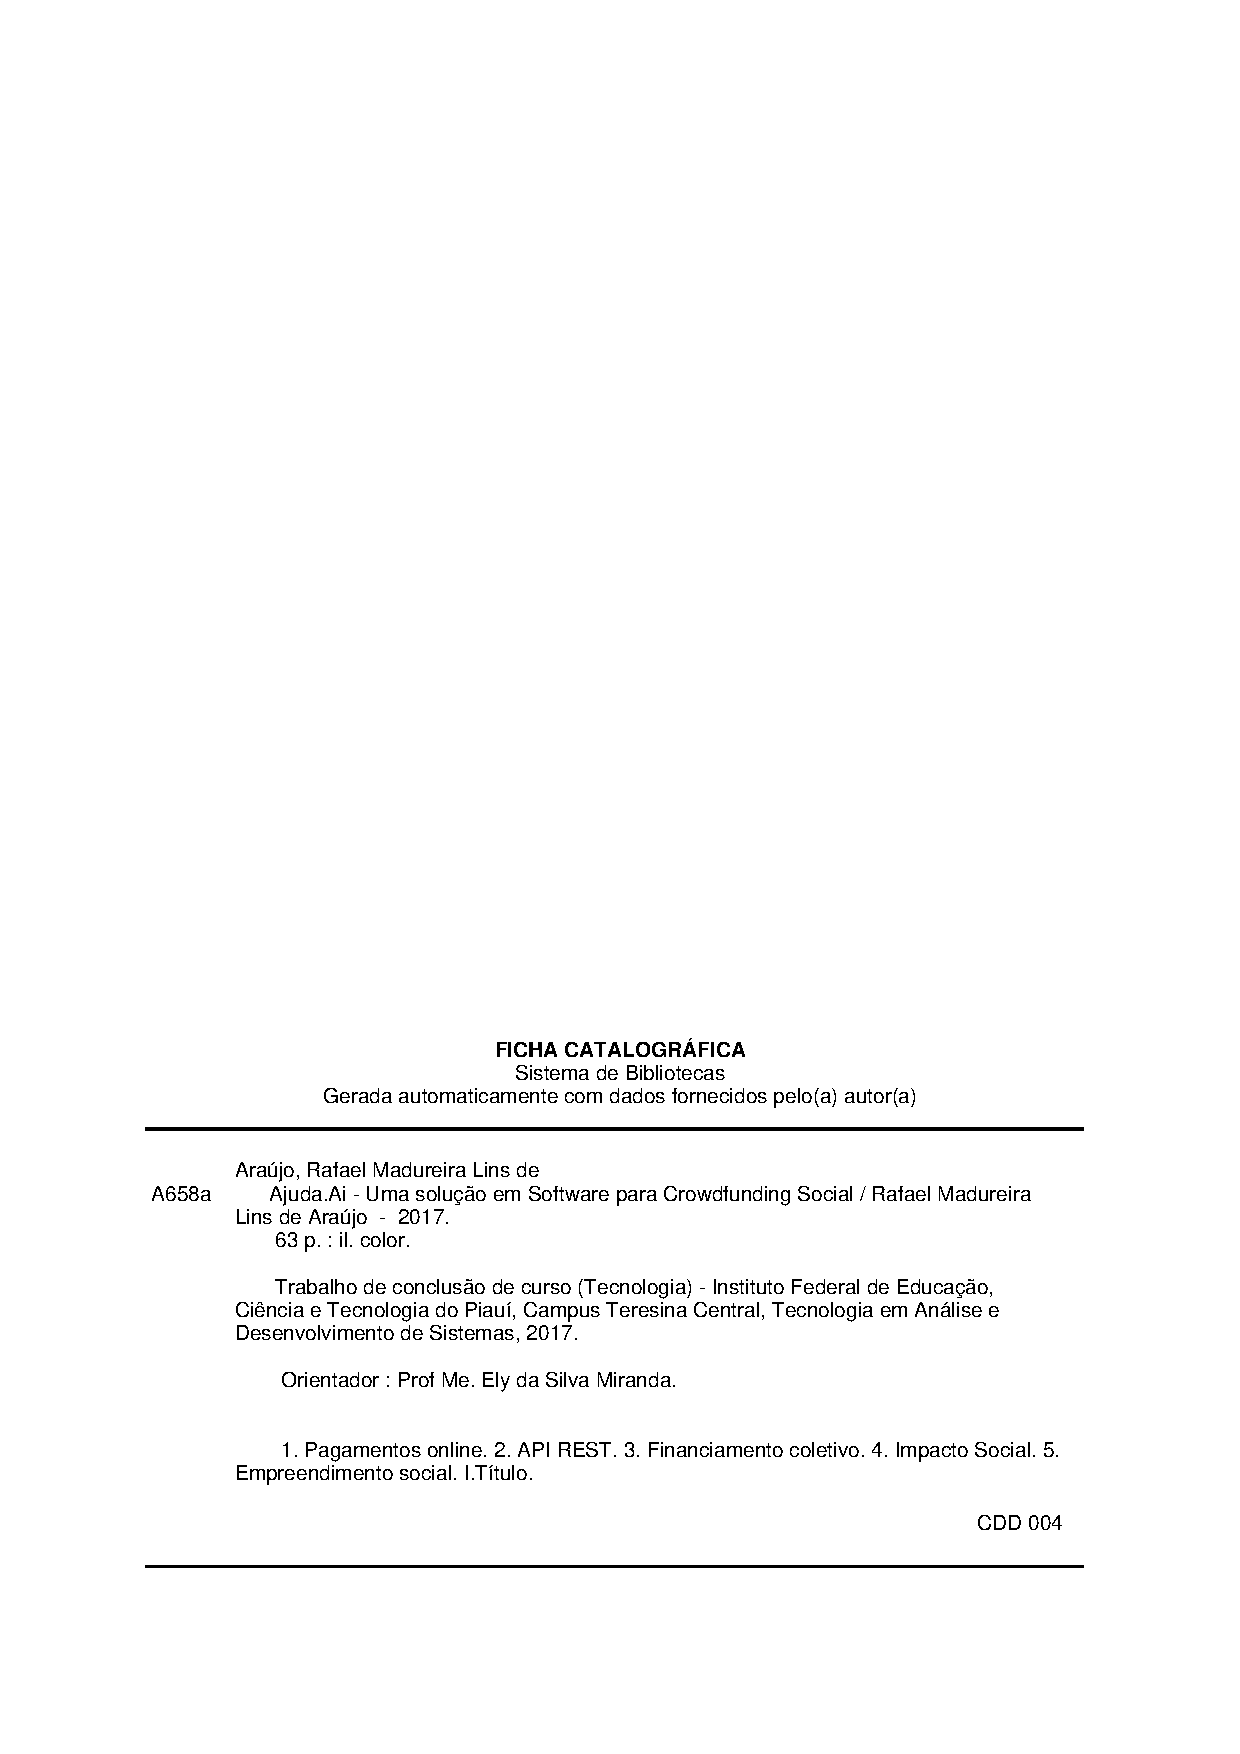
\includepdf{pre-textual/ficha-catalografica}


%% 03: Errata
%\input{pre-textual/errata}



%% 04: Folha de Aprovação
%\imprimirfolhadeaprovacao
% ----------------------------------------------------------
% Folha de Aprovação
% ----------------------------------------------------------

  \begin{center}
    {\ABNTEXchapterfont\MakeUppercase{\imprimirautor}}
    \vspace*{\fill}

    \vspace*{\fill}
    {\ABNTEXchapterfont\MakeUppercase{\imprimirtitulo}}
    \vspace*{\fill}

    \hspace{.45\textwidth}
    \begin{minipage}{.5\textwidth}
      \imprimirpreambulo
    \end{minipage}
    \vspace*{\fill}
  \end{center}
Aprovado em \dataapresentacao.
\\
  \begin{center}
  	

    
  	BANCA EXAMINADORA:
  \end{center}

  \setlength{\ABNTEXsignwidth}{12cm}
  \setlength{\ABNTEXsignskip}{0.5cm}
  \assinatura{\textbf{\imprimirorientador~(Orientador)} \\ Instituto Federal do Piauí (IFPI)}
  \assinatura{\textbf{\imprimirmembroum~(Membro Interno)} \\ Instituto Federal do Piauí (IFPI)}
  \assinatura{\textbf{\imprimirmembrodois~(Membro Externo)} \\ ClearTech}

  \begin{center}
    \vspace*{\fill}
    {\MakeUppercase{\imprimirlocal}}
    \par
    {\imprimirdata}
    \vspace*{1cm}
  \end{center}


%% Use esta se forem 4 membros na banca:
%\imprimirfolhadeaprovacaoduascolunas



%% 05: Dedicatória
%\include{pre-textual/dedicatoria}


%% 06: Epígrafe
%\input{pre-textual/epigrafe}

%% Título do Trabalho
\begin{center}{\ABNTEXchapterfont\bfseries\MakeUppercase{\imprimirtitulo}}
\end{center}


\flushright 
      
      \autornomecompleto\footnote{Graduando do Curso de Licenciatura em Computação. Instituto Federal de Educação, Ciência e Tecnologia do Piauí (IFPI), Campus Teresina Zona Sul.} \\
      \profnomecompleto \footnote{Professor orientador. Instituto Federal de Educação, Ciência e Tecnologia do Piauí (IFPI), Campus Teresina Zona Sul.}
      

\justifying 
%% 08: Resumo
% Definições básicas do resumo
\begin{adjustwidth}{-1cm}{-1cm}\vspace{\onelineskip}

%% Resumo

\begin{resumo}

O desempenho acadêmico no ensino médio público é fortemente condicionado por fatores sociológicos como pobreza, trabalho juvenil, exclusão digital e distorção idade-série, mas o acesso a microdados individuais de estudantes é restringido por barreiras legais e institucionais. Este trabalho propõe um modelo preditivo de tendência de desempenho acadêmico para estudantes da rede pública estadual do Piauí, fundamentado em fatores sociológicos e treinado sobre uma população sintética representativa do perfil de uma turma média dessa rede, construída pela própria pesquisa. Cada parâmetro de geração é rastreável a estatísticas oficiais e à literatura acadêmica, e o gerador incorpora mecanismos anti-deterministas: a assistência financeira estudantil é derivada de regra legal de elegibilidade, as vulnerabilidades interagem de forma não linear e perfis de resiliência acadêmica são preservados. Os indicadores acadêmicos observáveis correspondem a parciais do primeiro semestre letivo, e a variável-alvo representa a tendência de situação ao final do ano, rotulada pelos critérios de aprovação da Lei de Diretrizes e Bases da Educação Nacional. Sobre a base de três mil registros, três algoritmos de classificação e dois \textit{baselines} de referência foram comparados sob validação cruzada estratificada, com sobreamostragem confinada a cada partição de treino e teste estatístico pareado entre os modelos. O XGBoost obteve o melhor desempenho, com acurácia de 84,11\% (estatisticamente equivalente à \textit{Random Forest} e superior à \textit{Decision Tree} única e aos \textit{baselines}), e nenhum modelo cometeu erros entre as classes extremas. Após os sinais acadêmicos parciais, os atributos mais determinantes foram a distorção idade-série, o recebimento de assistência financeira, o trabalho juvenil e a renda per capita, recuperando o peso relativo atribuído aos fatores sociológicos no fenômeno gerador (evidência de validade metodológica da abordagem, cuja confirmação empírica depende da transposição a dados reais). Conclui-se que a articulação entre dados sintéticos rastreáveis e classificadores de conjunto constitui alternativa metodológica válida para o desenvolvimento de sistemas de alerta precoce em contextos de dados restritos.
\vspace{\onelineskip}
\noindent

\textbf{Palavras-chaves}: desempenho acadêmico; fatores sociológicos; dados sintéticos; aprendizado de máquina; ensino médio público.

\end{resumo}
\end{adjustwidth}


%% 09: Abstract/Resumo em língua estrangeira
\begin{adjustwidth}{-1cm}{-1cm}
%% Abstract (configurado para língua inglesa)
\begin{resumo}[Abstract]
\begin{otherlanguage*}{english}
Academic performance in Brazilian public high schools is strongly conditioned by sociological factors such as poverty, youth labor, digital exclusion, and age-grade distortion, yet access to individual student records is restricted by legal and institutional barriers. This work proposes a predictive model of academic performance trends for students of the state public school network of Piauí, grounded in sociological factors and trained on a synthetic population representative of the profile of an average class of that network. Every generation parameter is traceable to official statistics and academic literature, and the generator incorporates anti-deterministic mechanisms: student financial assistance is derived from a legal eligibility rule, vulnerabilities interact non-linearly, and academic resilience profiles are preserved. Observable academic indicators correspond to first-semester partial records, and the target variable represents the end-of-year trend, labeled according to Brazilian educational legislation on approval criteria. Over three thousand records, three classification algorithms and two reference \textit{baselines} were compared under stratified cross-validation, with oversampling confined to each training partition and paired statistical testing. XGBoost achieved 84.11\% accuracy, statistically equivalent to \textit{Random Forest} and superior to the single tree and to the \textit{baselines}, with no errors between the extreme classes. After the partial academic signals, the most determinant attributes were age-grade distortion, financial assistance, youth labor, and per capita income, recovering the relative weight of the sociological factors in the generating phenomenon. It is concluded that the articulation between traceable synthetic data and ensemble classifiers constitutes a valid methodological alternative for early-warning systems in restricted-data contexts.

\vspace{\onelineskip}
\noindent
\textbf{Keywords}: academic performance; sociological factors; synthetic data; machine learning; public high school.
\end{otherlanguage*}
\end{resumo}
\end{adjustwidth}



\hfill \break
Data de Aprovação: \dataapresentacao (Data de Apresentação do Artigo)
\hfill \break

%% 10: Lista de Ilustrações
\cleardoublepage
\input{pre-textual/lista-de-ilustracoes}

%% 11: Lista de Tabelas
\cleardoublepage
\input{pre-textual/lista-de-tabelas}

%% 12: Lista de Abreviaturas e Siglas
%%% Lista de Abreviaturas e Siglas
\begin{siglas}
  \item[AUC] \textit{Area Under the Curve} (Área sob a Curva)
  \item[BR] Brasil
  \item[CV] \textit{Cross-Validation} (Validação Cruzada)
  \item[DM] \textit{Data Mining} (Mineração de Dados)
  \item[EDM] \textit{Educational Data Mining} (Mineração de Dados Educacionais)
  \item[EM] Ensino Médio
  \item[IA] Inteligência Artificial
  \item[IBGE] Instituto Brasileiro de Geografia e Estatística
  \item[IFPI] Instituto Federal de Educação, Ciência e Tecnologia do Piauí
  \item[INEP] Instituto Nacional de Estudos e Pesquisas Educacionais Anísio Teixeira
  \item[KDD] \textit{Knowledge Discovery in Databases} (Descoberta de Conhecimento em Bancos de Dados)
  \item[LDB] Lei de Diretrizes e Bases da Educação Nacional
  \item[LIME] \textit{Local Interpretable Model-agnostic Explanations}
  \item[OvR] \textit{One-vs-Rest} (Um contra o Restante)
  \item[PI] Piauí
  \item[PNAD] Pesquisa Nacional por Amostra de Domicílios
  \item[RF] \textit{Random Forest} (Floresta Aleatória)
  \item[ROC] \textit{Receiver Operating Characteristic} (Característica de Operação do Receptor)
  \item[SHAP] \textit{SHapley Additive exPlanations}
  \item[SM] Salário Mínimo
  \item[SMOTE] \textit{Synthetic Minority Over-sampling Technique} (Técnica de Sobreamostragem Sintética da Minoria)
  \item[SVM] \textit{Support Vector Machine} (Máquina de Vetores de Suporte)
  \item[XGBoost] \textit{eXtreme Gradient Boosting}
\end{siglas}


%% 13: Lista de Símbolos
%\input{pre-textual/simbolos}

%% 14: Sumário (o asterisco retira o próprio sumário do sumário)
%\pdfbookmark[0]{\contentsname}{toc}
%\tableofcontents*
%\cleardoublepage



%% Indica que a partir daqui ficarão os elementos textuais (TCC em si)
\textual

%% %%%%%%%%%%%%%%%%%%%%%%%%%%%%%%%%%%% %%
%% Elementos Textuais (Capítulos)      %%
%% %%%%%%%%%%%%%%%%%%%%%%%%%%%%%%%%%%% %%
\pagestyle{empty} % Remover cabeçalho com titulo dos capítulos

%% Inclua aqui os capítulos que farão parte do Artigo
% ----------------------------------------------------------
% Introdução
% ----------------------------------------------------------
\chapter{Introdução}

O cenário atual da educação básica brasileira enfrenta desafios significativos relacionados à melhoria da qualidade do ensino e à redução dos índices de evasão, abandono e retenção \cite{dabreu2010, campos2024}. No ensino médio público, etapa final e mais crítica da educação básica, esses desafios assumem contornos estruturais: estima-se que apenas 74,3\% dos jovens brasileiros concluem o ensino médio até os 19 anos de idade, patamar que cai para 69,5\% entre jovens pretos, pardos e indígenas e para 70,5\% nos domicílios de menor renda \cite{todospelaeducacao2023}. Nesse contexto, a análise e a compreensão dos fatores que condicionam o sucesso ou o insucesso acadêmico dos estudantes tornam-se imprescindíveis para a implementação de estratégias pedagógicas e de políticas públicas eficazes.

A predição de desempenho acadêmico constitui um campo emergente na intersecção entre as ciências da educação e da computação, consolidado na literatura como Mineração de Dados Educacionais (EDM) \cite{baker2011, romero2010}. A possibilidade de identificar precocemente estudantes em trajetória de risco, a partir de dados demográficos, socioeconômicos e acadêmicos, representa uma oportunidade concreta para a gestão educacional baseada em evidências. A literatura sociológica, contudo, adverte que o desempenho escolar é um fenômeno multifatorial, fortemente condicionado pela origem social dos estudantes \cite{berlato2020, marturano2015}, o que exige que os modelos preditivos incorporem explicitamente os condicionantes sociológicos do rendimento (renda, trabalho juvenil, exclusão digital, distorção idade-série e políticas de permanência) sem, entretanto, reproduzir um determinismo social fatalista.

A dimensão dessas desigualdades é bem documentada pelas estatísticas oficiais, e assume contornos particularmente agudos no Piauí, objeto desta investigação. No estado, 45,3\% da população geral encontrava-se em situação de pobreza em 2023 \cite{ibgesis2024}, e a literatura demonstra que a pobreza entre crianças e adolescentes é sistematicamente superior à da população geral: cerca de 60\% dos estudantes brasileiros de 15 a 17 anos da rede pública vivem em domicílios com renda \textit{per capita} de até meio salário mínimo \cite{fadc2023}. A exclusão digital piauiense é acentuada: embora 92,5\% dos domicílios do estado disponham de acesso à internet, apenas 25,5\% possuem microcomputador ou \textit{tablet} (pouco mais da metade da média nacional de 40,9\%) \cite{ibgesidra2025tic, ibge2024tic}. A distorção idade-série (proporção de alunos com dois ou mais anos de atraso escolar) atingia 21,7\% na rede pública estadual do Piauí, após patamar histórico de 33,2\% \cite{inep2025, todospelaeducacaopiaui}; no mesmo período de consolidação das políticas de permanência, a taxa de abandono da rede recuou de 8,6\% para 0,5\% \cite{minutomt2026, santos2026}. A Tabela~\ref{tab:indicadores_em} consolida esses indicadores, que fundamentam quantitativamente a relevância do problema investigado.

\begin{table}[htb]
\centering
\caption{Indicadores educacionais e socioeconômicos que fundamentam o estudo.}
\label{tab:indicadores_em}
\begin{tabular}{p{6.2cm}cp{1.6cm}p{4.2cm}}
\toprule
\textbf{Indicador} & \textbf{Valor} & \textbf{Nível} & \textbf{Fonte} \\
\midrule
Conclusão do ensino médio até os 19 anos & 74,3\% & Brasil & \citeonline{todospelaeducacao2023} \\
Matrículas do ensino médio na rede pública & 82,0\% & Brasil & \citeonline{inep2025} \\
Estudantes de 15--17 anos da rede pública em situação de pobreza (renda \textit{per capita} $\le$ 0,5 SM) & $\sim$60\% & Brasil & \citeonline{fadc2023} \\
População em situação de pobreza (2023) & 45,3\% & Piauí & \citeonline{ibgesis2024} \\
Domicílios com acesso à internet & 92,5\% & Piauí & \citeonline{ibgesidra2025tic} \\
Domicílios com microcomputador ou \textit{tablet} & 25,5\% & Piauí & \citeonline{ibgesidra2025tic} \\
Distorção idade-série (rede pública estadual) & 21,7\% & Piauí & \citeonline{inep2025, todospelaeducacaopiaui} \\
Abandono no ensino médio (2022 $\rightarrow$ 2025) & 8,6\% $\rightarrow$ 0,5\% & Piauí & \citeonline{minutomt2026} \\
Estudantes do ensino médio de baixa renda que trabalham & 26,3\% & Brasil & \citeonline{berlato2020} \\
\bottomrule
\end{tabular}
\source{Elaborado pelo autor (2026).}
\end{table}

Delimitando-se o escopo desta investigação, o estudo concentra-se na elaboração de um modelo preditivo de \textbf{tendência de desempenho acadêmico} para estudantes do \textbf{ensino médio da rede pública estadual do Piauí}, fundamentado em fatores sociológicos. Em virtude das restrições de acesso a microdados individuais reais de estudantes (protegidos pela Lei Geral de Proteção de Dados e condicionados a autorizações institucionais e éticas cujos prazos de tramitação excedem o cronograma desta etapa da pesquisa), adotou-se uma estratégia metodologicamente validada pela literatura: a construção de uma \textbf{população sintética representativa do perfil de uma turma média} dessa rede, na qual cada distribuição é ancorada em estatísticas oficiais desagregadas para o Piauí sempre que disponíveis (IBGE, INEP, PNAD Contínua) e em estudos acadêmicos sobre os condicionantes sociais do desempenho escolar. Estudos recentes em EDM sustentam a validade preditiva de bases sintéticas de qualidade para o desenvolvimento e a validação de modelos de classificação \cite{kostopoulos2026, shabnam2025}, ressalvadas as diferenças entre técnicas de geração (discutidas no Referencial Teórico e retomadas nas limitações deste trabalho).

A problemática que orienta esta pesquisa emerge da constatação de que, apesar da crescente disponibilidade de dados educacionais e da consolidação das técnicas de aprendizado de máquina, há uma lacuna na construção de modelos preditivos que incorporem explicitamente, e com fundamentação estatística rastreável, os fatores sociológicos que condicionam o desempenho no ensino médio público. Questiona-se, assim: \textit{como construir um modelo de previsão de tendência de desempenho acadêmico para o ensino médio da rede pública estadual do Piauí, fundamentado em fatores sociológicos documentados pela literatura, e quais desses fatores se mostram mais determinantes na classificação dos estudantes?}

Dessa questão derivam quatro hipóteses de pesquisa, retomadas individualmente nas Considerações Finais:

\begin{description}
    \item[H1.] Classificadores de \textit{ensemble} (\textit{Random Forest} e XGBoost) superam a \textit{decision tree} única e os \textit{baselines} de referência (classificador majoritário e Regressão Logística) na predição da tendência de desempenho.
    \item[H2.] Os fatores sociológicos parametrizados no fenômeno gerador são recuperáveis pelos modelos como atributos de importância não redundante, mesmo na presença de indicadores acadêmicos diretos.
    \item[H3.] Sinais acadêmicos parciais do primeiro semestre são suficientes para prever a tendência do desfecho anual com desempenho substancialmente superior ao \textit{baseline} majoritário.
    \item[H4.] A regra legal de elegibilidade da assistência financeira estudantil produz, por si só, proporções coerentes de beneficiários entre cenários socioeconômicos contrastantes, sem parâmetro dedicado de calibração.
\end{description}

O presente trabalho propõe, portanto, a construção de um conjunto de dados sintéticos sociologicamente fundamentado e o desenvolvimento comparativo de modelos de classificação (\textit{Decision Tree}, \textit{Random Forest} e XGBoost) para prever a tendência de desempenho ao final do ano letivo (Aprovado, Em Risco ou Reprovado), a partir de sinais acadêmicos parciais do primeiro semestre e do contexto socioeconômico, identificando as variáveis mais determinantes e fornecendo subsídios para intervenções pedagógicas preventivas.

\section{Objetivo Geral}

Desenvolver um modelo preditivo de tendência de desempenho acadêmico para estudantes do ensino médio da rede pública estadual do Piauí, com base em fatores sociológicos, utilizando um conjunto de dados sintéticos fundamentado em estatísticas oficiais e na literatura acadêmica.

\section{Objetivos Específicos}

\begin{enumerate}
    \item Construir e parametrizar um gerador de dados sintéticos que reproduza o perfil demográfico, socioeconômico e acadêmico de uma turma média do ensino médio da rede pública estadual do Piauí, com rastreabilidade documentada entre cada parâmetro de distribuição e sua fonte estatística ou acadêmica, incluindo o nível de desagregação de cada fonte.
    \item Testar e avaliar comparativamente algoritmos de aprendizado de máquina (\textit{Decision Tree}, \textit{Random Forest} e XGBoost) frente a \textit{baselines} de referência, para identificar aquele com melhor desempenho na predição da tendência de rendimento acadêmico, sob tratamento adequado de desbalanceamento de classes, prevenção de vazamento de dados e teste estatístico pareado entre os modelos.
    \item Analisar e interpretar os resultados obtidos, verificando se os fatores sociológicos parametrizados no fenômeno gerador são recuperados pelos classificadores como atributos determinantes e discutindo suas implicações para intervenções pedagógicas e políticas de permanência, com salvaguardas explícitas contra vieses discriminatórios.
\end{enumerate}

% ----------------------------------------------------------
% Referencial Teórico
% ----------------------------------------------------------
\chapter{Referencial Teórico}

O referencial teórico está organizado de maneira a facilitar a compreensão dos conceitos que fundamentam a pesquisa. Inicialmente, discutem-se os fatores sociológicos que condicionam o desempenho escolar no ensino médio público brasileiro (fundamento da parametrização do conjunto de dados deste estudo) e o uso de dados sintéticos em Mineração de Dados Educacionais. Na sequência, apresenta-se a abordagem de descoberta de conhecimento em bancos de dados (KDD), seguida da aplicação da mineração de dados educacionais para a análise do desempenho acadêmico. Por fim, são detalhadas as técnicas de seleção de atributos, os métodos de validação de modelos, essenciais para a construção e a avaliação dos modelos preditivos, e os principais classificadores.

O desempenho acadêmico é um fenômeno multifatorial, influenciado por dimensões sociais, psicológicas, pedagógicas e individuais. Estudos como os apresentados por \citeonline{marturano2015} destacam que variáveis socioeconômicas, como renda familiar, acesso a recursos educacionais e contexto geográfico, desempenham papel crítico na determinação do sucesso discente.

No âmbito psicológico, fatores como motivação, autoeficácia e saúde mental têm sido amplamente discutidos. Segundo \citeonline{dabreu2010}, evidencia-se que a co-ocorrência de baixo desempenho escolar e problemas externalizantes sugere a influência de variáveis antecedentes, como condições adversas na família e baixo nível socioeconômico, corroborando a hipótese de que aspectos subjetivos devem ser considerados em análises preditivas. Além disso, características acadêmicas prévias são apontadas como preditores relevantes em modelos de inteligência artificial, conforme demonstrado em pesquisas com base em dados institucionais \cite{curi2006}.

A aplicação de técnicas de mineração de dados e \textit{machine learning} na educação tem ganhado destaque na literatura internacional e nacional. Algoritmos como \textit{decision trees} (árvores de decisão), redes neurais e regressão logística são frequentemente utilizados para identificar padrões em grandes conjuntos de dados educacionais \cite{baker2011}. Esses modelos permitem não apenas prever resultados acadêmicos, mas também mapear grupos de risco, facilitando intervenções personalizadas.

\section{Fatores Sociológicos do Desempenho Escolar no Ensino Médio Público}

A sociologia da educação demonstra, desde os estudos de reprodução social de Pierre Bourdieu, que o sistema escolar tende a reproduzir as condições sociais de origem dos estudantes, mais do que a transformá-las. Em investigação quantitativa com 3.287 estudantes do ensino médio público brasileiro, \citeonline{berlato2020} constataram que as diferenças entre agrupamentos de jovens estavam mais vinculadas às reproduções familiares e de classe social do que ao papel exercido pela escola, e que 26,3\% dos alunos de baixa renda precisavam conciliar trabalho e estudo. As desigualdades educacionais brasileiras, documentadas por \citeonline{wenczenovicz2023} e \citeonline{palominio2025}, expressam-se em barreiras estruturais de acesso, permanência e êxito escolar que incidem de forma desproporcional sobre estudantes pobres, pretos, pardos e residentes nas regiões Norte e Nordeste.

Entre os condicionantes mensuráveis do desempenho, destacam-se quatro eixos documentados pelas estatísticas oficiais e pela literatura. O primeiro é a \textbf{pobreza}: cerca de 60\% dos estudantes de 15 a 17 anos da rede pública brasileira vivem em domicílios com renda per capita de até meio salário mínimo \cite{fadc2023}; no Piauí, 45,3\% da população geral encontrava-se em situação de pobreza em 2023 \cite{ibgesis2024}, sendo que a pobreza infanto-juvenil é sistematicamente superior à da população geral \cite{fadc2023}. O segundo é a \textbf{exclusão digital}, que no Piauí assume caráter qualitativo: 92,5\% dos domicílios dispõem de acesso à internet, mas apenas 25,5\% possuem microcomputador ou \textit{tablet} (contra 40,9\% na média nacional), de modo que os acessos dependem majoritariamente de aparelhos celulares, comprometendo atividades que exigem proficiência digital \cite{ibgesidra2025tic, ibge2024tic}. O terceiro é a \textbf{distorção idade-série}, percentual de alunos com dois ou mais anos de atraso em relação à idade recomendada: associada ao gênero masculino, à matrícula em áreas de pobreza e à necessidade de geração de renda \cite{lima2013, chiapinoto2024}, a distorção desloca a distribuição etária das turmas para a direita, com cauda longa que se estende até os 24 anos. No Piauí, o indicador recuou de 33,2\% para 21,7\% na rede estadual \cite{inep2025, todospelaeducacaopiaui}. O quarto é o \textbf{trabalho juvenil}, que subtrai tempo de estudo e está diretamente associado ao abandono temporário e à retenção \cite{berlato2020, campos2024}; no Piauí, a taxa de trabalho infantil (5 a 17 anos) situava-se entre 6,8\% e 8,6\% no biênio 2023--2024 \cite{mte2024trabalho} (conceito adjacente, porém distinto, do estudante de ensino médio que trabalha).

Em contraposição a esses fatores de risco, as \textbf{políticas públicas de permanência} operam como mecanismo de reversão de tendência. O programa Pé-de-Meia, instituído pela Lei nº 14.818, de 2024, constitui incentivo financeiro-educacional na modalidade de poupança destinado a estudantes do ensino médio público de 14 a 24 anos, inscritos em famílias do Cadastro Único com renda per capita de até meio salário mínimo, condicionado à frequência mínima de 80\% das aulas \cite{brasil2024lei14818, mds2024cadunico}. Análises iniciais do programa indicam forte efeito de retenção sobre estudantes em vulnerabilidade \cite{santos2026}: no Piauí, onde o programa atende 187.620 estudantes, a taxa de abandono da rede estadual recuou de 8,6\% para 0,5\% no período de consolidação das políticas de permanência \cite{todospelaeducacaopiaui, inep2025, minutomt2026}. Programas estaduais anteriores, como o Poupança Jovem Piauí, exibiram efeito análogo \cite{palominio2025}.

A literatura adverte, contudo, contra o \textbf{determinismo social} em modelos preditivos educacionais: vulnerabilidade severa não implica insucesso inevitável. O caso da Unidade Escolar Augustinho Brandão, em Cocal dos Alves (PI) (escola pública que atende comunidade de baixa renda e superou milhares de escolas públicas e privadas no Exame Nacional do Ensino Médio), ilustra que a sinergia entre engajamento discente e infraestrutura pedagógica pode romper as barreiras da origem social \cite{seducpi}. Modelos preditivos responsáveis devem, portanto, capturar interações não lineares (como o efeito de reversão da assistência financeira) e tolerar perfis de resiliência acadêmica, sem penalizar fatalisticamente os estudantes vulneráveis, uma diretriz incorporada à construção do conjunto de dados deste estudo.

\section{Dados Sintéticos em Mineração de Dados Educacionais}

O acesso a microdados educacionais individuais é crescentemente restringido por legislações de proteção de dados pessoais e por trâmites institucionais e éticos. Nesse cenário, a geração de dados sintéticos (registros artificiais que preservam as distribuições estatísticas e as relações entre variáveis da população de interesse) consolidou-se como alternativa metodológica válida em EDM \cite{kostopoulos2026}. Em avaliação comparativa (\textit{benchmarking}) de modelos generativos estatísticos e profundos aplicados a dados estudantis, \citeonline{kostopoulos2026} demonstram que bases sintéticas de qualidade preservam a utilidade preditiva dos dados originais, com a vantagem de eliminar riscos de reidentificação de estudantes.

Resultados convergentes são reportados por \citeonline{shabnam2025}, que compararam dados reais, sintéticos e híbridos na predição de desempenho de estudantes com algoritmos de regressão e \textit{ensemble}: os dados sintéticos igualaram os reais em capacidade preditiva, e conjuntos híbridos alcançaram acurácia de até 87,76\%. Técnicas baseadas em redes adversárias generativas condicionais e transformadores tabulares atingem entre 96\% e 98\% de equivalência preditiva em relação aos dados autênticos \cite{kostopoulos2026, shabnam2025}, sustentando o uso de bases sintéticas para o desenvolvimento e a validação de modelos de classificação quando o acesso primário é vedado.

É necessário, contudo, distinguir duas famílias de dados sintéticos com estatutos epistemológicos diferentes. Os estudos de equivalência preditiva citados referem-se a dados sintéticos \textbf{derivados de microdados reais}: modelos generativos (estatísticos ou profundos, como redes adversárias condicionais e transformadores tabulares) são ajustados sobre uma base autêntica e produzem réplicas que preservam suas distribuições conjuntas \cite{kostopoulos2026, shabnam2025}. Este trabalho, por indisponibilidade de microdados, situa-se na segunda família: a \textbf{simulação baseada em regras}, na qual as distribuições marginais são parametrizadas a partir de estatísticas agregadas oficiais e as relações entre variáveis são especificadas pelo pesquisador com fundamento na literatura. Nessa família, a validade da base não é herdada de dados reais, mas depende integralmente da qualidade da parametrização e da auditabilidade das fontes, e as métricas obtidas medem a capacidade dos classificadores de recuperar um fenômeno cuja estrutura é, em parte, conhecida por construção.

Dessa distinção decorrem os dois requisitos que orientam a metodologia deste trabalho: (i) a \textbf{rastreabilidade} entre cada parâmetro de geração e sua fonte estatística ou acadêmica (incluindo o nível de desagregação da fonte), de modo que as distribuições simuladas sejam auditáveis; e (ii) a \textbf{não trivialidade} do problema resultante, garantida pela injeção de variância estocástica e de casos-limite que impeçam os classificadores de memorizar a regra geradora.

\section{Descoberta de Conhecimento em Bancos de Dados (KDD)}

Para lidar com o desafio da crescente quantidade e volume de dados disponíveis, \citeonline{fayyad1996} propuseram o processo de Descoberta de Conhecimento em Banco de Dados (KDD (\textit{Knowledge Discovery in Databases})). Esse processo visa identificar padrões explicáveis nos dados, permitindo interpretações e previsões para auxiliar na tomada de decisões \cite{baker2011}.

O processo de KDD é dinâmico e iterativo, podendo exigir retornos a etapas anteriores conforme novas descobertas são feitas \cite{fayyad1996}. A Figura~\ref{fig:kdd} apresenta a visão geral de suas etapas.

\begin{figure}[htb]
\centering
\caption{Visão geral das etapas que compõem o processo de KDD.}
\label{fig:kdd}
\begin{mermaid}[width=0.85\textwidth,keepaspectratio]
flowchart LR
  A[("Base de<br/>dados")] --> B["Selecao<br/>de dados"]
  B --> C["Pre-<br/>processamento"]
  C --> D["Transformacao<br/>dos dados"]
  D --> E["Mineracao<br/>de dados"]
  E --> F["Interpretacao<br/>dos resultados"]
  F --> G[("Conhecimento")]
  F -. iteracao .-> B
\end{mermaid}
\source{Adaptado de \citeonline{fayyad1996}.}
\end{figure}

Ele é composto pelas seguintes etapas:

\begin{enumerate}
    \item \textbf{Seleção de Dados:} Define-se a origem das informações e selecionam-se as características relevantes para a mineração de dados.
    \item \textbf{Pré-processamento:} Garante a qualidade dos dados, identificando e corrigindo inconsistências, como valores ausentes, \textit{outliers} e erros.
    \item \textbf{Transformação dos Dados:} Converte os dados para formatos mais adequados à análise, incluindo discretização de variáveis contínuas e criação de novas variáveis.
    \item \textbf{Mineração de Dados:} Utiliza algoritmos e técnicas estatísticas para identificar padrões e relações nos dados, sendo a etapa central do processo.
    \item \textbf{Interpretação dos Resultados:} Analisa as descobertas para apoiar a tomada de decisões.
\end{enumerate}

O KDD inicia-se com uma base de dados relacionada ao objetivo da análise e gera conhecimento aplicável à tomada de decisão. Sendo um processo cíclico, ele pode ser aprimorado continuamente com novas iterações \cite{maimon2010}.

\section{Mineração de Dados Educacionais}

A Mineração de Dados (\textit{Data Mining}, DM) emerge como resposta fundamental às limitações da análise manual frente ao crescimento do volume de dados. Esta abordagem transcende as fronteiras de diversas áreas, incluindo estatística, aprendizado de máquina e visualização de dados, constituindo elemento essencial do processo de KDD \cite{castro2016}.

No contexto educacional, a aplicação específica denomina-se Mineração de Dados Educacionais (\textit{Educational Data Mining}, EDM). Esta vertente especializada explora informações sobre comportamentos, avaliações e conquistas dos alunos \cite{costa2012}. A EDM estrutura-se conforme as necessidades do usuário final, seja ele aluno, educador, administrador ou pesquisador \cite{romero2010}.

\citeonline{pena2014} identificou diversos objetivos gerais associados ao processo de EDM, incluindo a modelagem de aluno, a análise do comportamento discente e a previsão do desempenho acadêmico, que visa antecipar notas finais e outros resultados de aprendizagem com base nos dados das atividades realizadas durante o curso.

Nessa linha, a literatura de EDM destaca o valor preditivo dos \textbf{sinais de engajamento contínuo}: além das notas de provas e da frequência, o desempenho e a regularidade nas atividades avaliativas ao longo do período capturam a dimensão comportamental do engajamento escolar (um construto multidimensional que antecede o desfecho acadêmico) \cite{fredricks2004}. \citeonline{costa2012} demonstram que a combinação de dados demográficos coletados no início do período com métricas de engajamento pedagógico (notas de avaliações contínuas e frequência) provê predições com acurácia superior a 80\% ainda em estágio inicial do curso (fundamento da inclusão, neste trabalho, de variáveis de desempenho e de entrega de atividades como sinais parciais do primeiro semestre).

\section{Técnicas de Seleção de Atributos}

A seleção de características desempenha papel fundamental na otimização de modelos preditivos. Conforme \citeonline{liu2007}, existem três categorias principais de técnicas: \textit{Filter}, \textit{Wrapper} e \textit{Embedded}. Cada abordagem apresenta equilíbrio distinto entre eficiência computacional e qualidade dos resultados.

A abordagem \textit{Embedded} integra a seleção de características ao processo de treinamento do modelo, constituindo parte fundamental de algoritmos como \textit{Decision Tree} e \textit{Random Forest}. A técnica \textit{Filter} remove características sem utilidade, apresentando baixo custo computacional. A abordagem \textit{Wrapper} permite experimentar subconjuntos de características em conjunto com o algoritmo específico, embora demande maior processamento.

\section{Métodos de Validação de Modelos}

A validação cruzada (\textit{Cross-Validation}) representa uma abordagem robusta para avaliação da capacidade de generalização de modelos preditivos. Esta técnica divide os dados em \textit{k} subconjuntos, utilizando cada um como conjunto de teste enquanto os demais funcionam como treinamento. A configuração \textit{k=10} é frequentemente adotada \cite{geron2019}.

Uma abordagem alternativa é o método \textit{Holdout}, que consiste na divisão dos dados em conjuntos distintos de treinamento e teste, fornecendo uma estimativa do erro em relação a dados desconhecidos \cite{geron2019}.

\section{Desbalanceamento de Dados e Estratégias de Correção}

O desbalanceamento de dados ocorre quando um conjunto apresenta quantidade significativamente maior de instâncias em uma classe comparativamente a outra. Para superar este desafio, técnicas de balanceamento são empregadas, destacando-se a subamostragem e a sobreamostragem \cite{he2009}.

A sobreamostragem via SMOTE (\textit{Synthetic Minority Oversampling Technique}) emprega abordagens estatísticas para gerar instâncias minoritárias sintéticas, enriquecendo a diversidade dos dados sem mera replicação \cite{chawla2002}. Contudo, a aplicação incorreta do SMOTE constitui uma das fontes mais recorrentes de vazamento de dados (\textit{data leakage}) em estudos de aprendizado de máquina \cite{madugula2026}. O vazamento ocorre quando a sobreamostragem é aplicada sobre o conjunto de dados completo antes da divisão entre treino e teste, fazendo com que informações sintéticas geradas a partir de instâncias de teste contaminem o conjunto de treinamento. Para mitigar esse problema, a técnica deve ser confinada estritamente ao conjunto de treinamento dentro de cada partição da validação cruzada, utilizando-se \textit{pipelines} que encapsulam o SMOTE como etapa interna ao \textit{fold}, uma abordagem adotada neste trabalho por meio do \texttt{imblearn.Pipeline} \cite{madugula2026}.

\section{Decision Trees}

\textit{Decision Trees} (árvores de decisão) constituem classificadores que, a partir de um vetor de atributos, definem por meio de trajetórias decisórias um resultado final \cite{russel2013}. Na aplicação voltada ao desempenho acadêmico, este modelo revela os fatores subjacentes que influenciam as previsões, permitindo interpretação clara dos processos decisórios \cite{grus2016}. A Figura~\ref{fig:arvore_decisao} ilustra a estrutura genérica do classificador.

\begin{figure}[htb]
\centering
\caption{Estrutura genérica de uma \textit{decision tree}.}
\label{fig:arvore_decisao}
\begin{mermaid}[width=0.85\textwidth,keepaspectratio]
flowchart TD
  A{"No raiz:<br/>atributo X1"} -->|"condicao a"| B{"No interno:<br/>atributo X2"}
  A -->|"condicao b"| C{"No interno:<br/>atributo X3"}
  B -->|"sim"| D["Folha:<br/>Classe 1"]
  B -->|"nao"| E["Folha:<br/>Classe 2"]
  C -->|"sim"| F["Folha:<br/>Classe 2"]
  C -->|"nao"| G["Folha:<br/>Classe 3"]
\end{mermaid}
\source{Elaborado pelo autor (2026), com base em \citeonline{russel2013}.}
\end{figure}

Como se observa na Figura~\ref{fig:arvore_decisao}, a classificação parte de um nó raiz, no qual o atributo mais discriminante é avaliado, e percorre nós internos com condições sucessivas sobre os demais atributos, até alcançar um nó folha, que atribui a classe final à instância. Essa estrutura hierárquica de decisões é o que torna o modelo diretamente interpretável: cada predição corresponde a uma trajetória legível de regras.

\section{Random Forest}

A \textit{Random Forest} (Floresta Aleatória) é uma abordagem robusta que agrega diversas \textit{decision trees} para tarefas de classificação e regressão. Cada árvore é construída independentemente a partir de uma amostra aleatória do conjunto de dados \cite{artero2009}.

No processo de treinamento, utiliza-se a técnica de \textit{bagging} (\textit{bootstrap aggregating}), que gera múltiplas amostras por meio de reamostragem com reposição. Em cada divisão de nó, seleciona-se aleatoriamente um subconjunto de atributos para avaliação, contribuindo para diminuir tanto o viés quanto a variância do modelo \cite{geron2019}. A diversidade induzida pela aleatoriedade dupla (amostras \textit{bootstrap} e subconjuntos de características) é o mecanismo central que confere à \textit{Random Forest} resistência ao sobreajuste (\textit{overfitting}) e capacidade de capturar interações complexas entre variáveis \cite{denisko2018}. A Figura~\ref{fig:random_forest} ilustra a estrutura do \textit{ensemble}.

\begin{figure}[htb]
\centering
\caption{Estrutura genérica de uma \textit{Random Forest}.}
\label{fig:random_forest}
\begin{mermaid}[width=0.85\textwidth,keepaspectratio]
flowchart TD
  A[("Conjunto de<br/>treinamento")] --> B1["Amostra<br/>bootstrap 1"]
  A --> B2["Amostra<br/>bootstrap 2"]
  A --> B3["Amostra<br/>bootstrap n"]
  B1 --> C1{{"Arvore 1"}}
  B2 --> C2{{"Arvore 2"}}
  B3 --> C3{{"Arvore n"}}
  C1 --> D["Votacao<br/>majoritaria"]
  C2 --> D
  C3 --> D
  D --> E["Predicao<br/>final"]
\end{mermaid}
\source{Elaborado pelo autor (2026), com base em \citeonline{geron2019}.}
\end{figure}

A Figura~\ref{fig:random_forest} evidencia o funcionamento do \textit{ensemble}: a partir do conjunto de treinamento, são extraídas múltiplas amostras \textit{bootstrap}, cada uma originando uma árvore treinada de forma independente; na predição, as saídas individuais das árvores são combinadas por votação majoritária, produzindo a classificação final com variância reduzida em relação a uma árvore única.

\section{Gradient Boosting e XGBoost}

Enquanto a \textit{Random Forest} baseia-se no paradigma de \textit{bagging} (construindo árvores independentes em paralelo e combinando-as por votação), o \textit{Gradient Boosting} adota uma estratégia sequencial, na qual cada nova árvore é treinada para corrigir os erros residuais das anteriores. Essa abordagem foi formalizada matematicamente por \citeonline{friedman2001}, que demonstrou que o \textit{boosting} pode ser interpretado como um algoritmo de otimização numérica no espaço de funções, utilizando o gradiente descendente para minimizar uma função de perda arbitrária.

O XGBoost (\textit{eXtreme Gradient Boosting}) constitui uma implementação otimizada e regularizada do \textit{Gradient Boosting}, proposta por \citeonline{chen2016}. O algoritmo incorpora dois avanços fundamentais em relação à formulação original de Friedman. Primeiro, emprega uma aproximação de Taylor de segunda ordem da função de perda, permitindo capturar a curvatura do erro e direcionar a otimização com maior precisão: enquanto o \textit{Gradient Boosting} clássico utiliza apenas a informação do gradiente de primeira ordem, o XGBoost incorpora também o Hessiano, isto é, a derivada de segunda ordem da função de perda em relação à predição. Segundo, introduz um termo de regularização explícito que penaliza a complexidade das árvores, controlando simultaneamente o número de folhas e a magnitude dos pesos, o que reduz o sobreajuste de forma mais eficaz que a mera limitação de profundidade \cite{chen2016}.

Adicionalmente, o XGBoost apresenta otimizações algorítmicas que o tornam particularmente eficiente em cenários com dados esparsos e valores ausentes, incluindo um algoritmo de divisão ponderada por quantis e tratamento nativo de registros incompletos (características relevantes para domínios educacionais, nos quais lacunas de informação são frequentes) \cite{chen2016}.

\section{Métricas de Avaliação para Classificação Multiclasse}

A avaliação do desempenho de modelos preditivos em cenários com classes desbalanceadas exige métricas que vão além da acurácia simples. Em problemas nos quais uma ou mais classes são sub-representadas (como é o caso da classe de alunos \textit{Reprovados} frente aos \textit{Aprovados}), a acurácia tende a favorecer a classe majoritária, mascarando deficiências críticas na identificação dos grupos minoritários \cite{he2009}.

Diante desse desafio, emprega-se o F1-Score, métrica que combina precisão e \textit{recall} por meio da média harmônica, penalizando modelos que sacrificam uma das dimensões em detrimento da outra. Para cenários multiclasse, adota-se a variante ponderada (\textit{weighted F1-Score}), que calcula o F1 de cada classe individualmente e agrega os resultados ponderando-os pela proporção de instâncias reais de cada classe no conjunto de dados. Essa variante é particularmente adequada quando as frequências das classes refletem a distribuição natural do fenômeno estudado (como ocorre com o desempenho acadêmico), pois atribui maior peso às classes mais populosas sem ignorar o desempenho nas minoritárias.

Complementarmente, a análise por meio da Curva ROC (\textit{Receiver Operating Characteristic}) e da Área sob a Curva (AUC) constitui uma abordagem consolidada para avaliação de classificadores \cite{fawcett2006}. Em problemas binários, a curva ROC plota a taxa de verdadeiros positivos em função da taxa de falsos positivos para diferentes limiares de decisão, e a AUC sintetiza essa informação em um escalar no intervalo $[0, 1]$. Para o contexto multiclasse, \citeonline{hand2001} propuseram uma generalização do AUC por meio da estratégia \textit{One-vs-Rest} (OvR), na qual cada classe é tratada como positiva contra a união das demais, produzindo uma curva ROC por classe. A média ponderada das AUCs individuais fornece uma medida global da capacidade discriminativa do modelo, mantendo a interpretabilidade do caso binário \cite{hand2001}.

\section{Baselines de Referência e Comparação Estatística de Classificadores}

A magnitude de uma métrica, isoladamente, não informa se um modelo é bom: um classificador com 80\% de acurácia pode ser trivial se a classe majoritária representar 80\% das instâncias. Por isso, boas práticas de avaliação recomendam a inclusão de \textbf{\textit{baselines} de referência}: um classificador trivial que sempre prediz a classe majoritária, estabelecendo o piso de desempenho do problema, e um modelo linear simples (como a Regressão Logística), que quantifica a parcela do fenômeno explicável por relações lineares. A diferença entre os modelos de interesse e esses \textit{baselines} mede a contribuição efetiva da capacidade não linear dos algoritmos \cite{geron2019}.

Adicionalmente, diferenças numéricas entre classificadores podem decorrer da variabilidade amostral das partições de avaliação. Para verificar se a diferença observada entre dois modelos é estatisticamente significativa, \citeonline{demsar2006} recomenda o \textbf{teste pareado de postos sinalizados de Wilcoxon} sobre os resultados das mesmas partições de validação cruzada: por ser não paramétrico, o teste não pressupõe normalidade das diferenças, sendo mais robusto que o teste $t$ pareado para comparação de classificadores. Quando o valor-$p$ excede o nível de significância adotado, a diferença entre os modelos não pode ser distinguida da flutuação amostral, e conclusões de superioridade devem ser evitadas ou moderadas.

% ----------------------------------------------------------
% Trabalhos Correlatos
% ----------------------------------------------------------
\chapter{Trabalhos Correlatos}

A previsão do desempenho escolar e o combate à evasão utilizando algoritmos de aprendizado de máquina têm sido amplamente investigados na literatura nacional. Para contextualizar a presente proposta e identificar o estado da arte na área de Mineração de Dados Educacionais (EDM), foram selecionados trabalhos de referência cujas características estruturais de modelagem tangenciam as abordagens deste estudo.

\citeonline{silva2019} avaliaram o desempenho de estudantes universitários utilizando regressão logística e \textit{decision trees}. Os autores destacaram que variáveis socioeconômicas (como renda e nível de escolaridade dos pais) operaram como fortes determinantes de retenção nos períodos acadêmicos iniciais.

Por sua vez, \citeonline{costa2012} propuseram um sistema preditivo voltado à detecção de alunos em risco de reprovação em disciplinas introdutórias de programação por meio de algoritmos de classificação Bayesiana e \textit{decision trees}. Constatou-se que o uso de dados demográficos no início do semestre combinado a dados de engajamento pedagógico provê predições com acurácia superior a 80\%.

Nessa linha de análise, \citeonline{baker2011} e \citeonline{romero2010} discutiram a importância da integração de múltiplas fontes de dados (registros acadêmicos e bases contextuais) e o emprego de técnicas para contornar problemas de desbalanceamento de classes, como o SMOTE. Argumenta-se que a correção do desbalanceamento propicia uma sensibilidade substancialmente maior no mapeamento de alunos em risco de evasão.

A Tabela~\ref{tab:trabalhos_correlatos} resume as similaridades e contrastes metodológicos entre as principais iniciativas da literatura e a presente pesquisa.

\begin{table}[htb]
\centering
\caption{Comparação metodológica entre trabalhos correlatos da literatura e o presente estudo.}
\label{tab:trabalhos_correlatos}
\begin{tabular}{p{3.5cm}p{3.2cm}p{4.2cm}p{4cm}}
\toprule
\textbf{Trabalho / Autor} & \textbf{Algoritmos Usados} & \textbf{Principais Atributos} & \textbf{Relação com este Trabalho} \\
\midrule
\citeonline{silva2019} & Regressão Logística, \textit{Decision Tree} & Sociodemográficos (renda, escolaridade familiar, cota) & Compartilha o eixo socioeconômico, aqui expandido com conectividade, trabalho e assistência financeira. \\
\citeonline{costa2012} & Naive Bayes, \textit{Decision Tree} & Notas de avaliações contínuas, frequência, dados demográficos & Adota a formulação de métricas de engajamento e a classificação multiclasse do rendimento discente. \\
\citeonline{pena2014} & Redes Neurais Alternativas, SVM, \textit{Random Forest} & Histórico escolar prévio, taxas de evasão municipais & Utiliza \textit{Random Forest} como referencial robusto, integrando-a com técnicas avançadas de SMOTE. \\
\textbf{Este Estudo (rede pública estadual do PI)} & \textbf{\textit{Decision Tree}, \textit{Random Forest}, XGBoost + \textit{baselines}} & \textbf{Fatores sociológicos (renda \textit{per capita}, trabalho, exclusão digital, distorção idade-série, Pé-de-Meia) + sinais acadêmicos parciais do 1º semestre (nota, frequência, atividades)} & \textbf{Constrói o próprio conjunto de dados sintéticos com rastreabilidade parâmetro--fonte; SMOTE dentro do CV k=10; alvo de tendência de desempenho anual (critérios da LDB), não evasão.} \\
\bottomrule
\end{tabular}
\source{Elaborado pelo autor (2026).}
\end{table}

A Tabela~\ref{tab:trabalhos_correlatos} evidencia que, embora os trabalhos correlatos compartilhem algoritmos e famílias de atributos com esta pesquisa, nenhum deles combina a construção fundamentada do próprio conjunto de dados com a predição de tendência de desempenho no ensino médio público estadual, lacuna que o presente estudo busca preencher.

Diferentemente dos trabalhos correlatos apresentados (majoritariamente voltados à predição de evasão ou reprovação em disciplinas do ensino superior, a partir de bases institucionais preexistentes), o presente estudo une, em uma única investigação, a \textbf{construção do conjunto de dados} e a \textbf{modelagem preditiva}: o conjunto de dados sintéticos é gerado com parametrização sociologicamente fundamentada e rastreável às fontes oficiais, e a variável-alvo é a \textbf{tendência de desempenho acadêmico} (e não a evasão) de estudantes do ensino médio da rede pública estadual do Piauí. Essa combinação permite avaliar de forma controlada o peso relativo dos fatores sociológicos na classificação, algo inviável em bases institucionais nas quais tais variáveis são incompletas ou inacessíveis.

% ----------------------------------------------------------
% Metodologia
% ----------------------------------------------------------
\chapter{Metodologia}

A metodologia deste trabalho fundamenta-se no processo de Descoberta de Conhecimento em Bancos de Dados (KDD), estruturado para desenvolver um modelo preditivo de tendência de desempenho acadêmico de estudantes do ensino médio da rede pública estadual do Piauí, com base em fatores sociológicos. Como o acesso a microdados individuais reais é vedado por restrições legais e institucionais, a fonte de dados do estudo é um conjunto sintético construído pelo próprio trabalho (uma população representativa do perfil de uma turma média dessa rede), no qual cada distribuição é parametrizada a partir de estatísticas oficiais desagregadas para o Piauí sempre que disponíveis (IBGE, INEP, PNAD Contínua) e da literatura acadêmica apresentada no Referencial Teórico. Trata-se de simulação baseada em regras, nos termos da distinção estabelecida no Referencial: a validade da base depende da qualidade da parametrização e da auditabilidade das fontes, requisitos operacionalizados pela matriz de rastreabilidade apresentada adiante.

\section{Classificação da Pesquisa}

Seguindo os referenciais metodológicos de \citeonline{gil2017}, esta pesquisa classifica-se, quanto à natureza, como aplicada; quanto à abordagem, como quantitativa; e, quanto aos objetivos, como exploratória e descritiva. Quanto aos procedimentos técnicos, combina o levantamento documental (utilizado na fundamentação estatística dos parâmetros de geração, a partir de relatórios oficiais e estudos acadêmicos publicados) com a pesquisa experimental, materializada na variação controlada de parâmetros do gerador de dados e na comparação sistemática de algoritmos de classificação sob condições idênticas de treinamento e avaliação.

\section{Procedimentos Técnicos}

Os procedimentos técnicos organizam-se em etapas sequenciais e reprodutíveis, executadas sob semente aleatória fixa e parâmetros documentados: geração dos dados sintéticos (com exportação da matriz de rastreabilidade parâmetro--fonte), pré-processamento, treinamento e otimização dos três classificadores e dos \textit{baselines} de referência, avaliação por \textit{holdout} e validação cruzada com teste estatístico pareado, e análise dos resultados. A Figura~\ref{fig:pipeline} apresenta a visão geral das etapas.

\begin{figure}[htb]
\centering
\caption{Etapas metodológicas do estudo.}
\label{fig:pipeline}
\begin{mermaid}[height=0.55\textheight,keepaspectratio]
flowchart LR
  subgraph S1[" "]
    direction TB
    A["Fundamentacao estatistica e academica<br/>(IBGE, INEP, PNAD, literatura)"] --> B["Geracao de dados sinteticos<br/>+ matriz de rastreabilidade"]
    B --> C["Pre-processamento<br/>e feature engineering"]
    C --> D["Divisao treino/teste<br/>(70/30) estratificada"]
  end
  subgraph S2[" "]
    direction TB
    E["SMOTE dentro<br/>de cada fold"] --> F["GridSearchCV (k=5):<br/>Arvore de Decisao, RF, XGBoost<br/>+ baselines de referencia"]
    F --> G["Avaliacao: holdout + CV k=10<br/>(Acuracia, F1, Precisao, AUC-ROC)<br/>+ teste pareado de Wilcoxon"]
    G --> H["Analise dos resultados:<br/>importancias, matrizes de confusao,<br/>curvas ROC"]
  end
  S1 --> S2
  style S1 fill:none,stroke:#999,stroke-dasharray:4
  style S2 fill:none,stroke:#999,stroke-dasharray:4
\end{mermaid}
\source{Elaborado pelo autor (2026).}
\end{figure}

A Figura~\ref{fig:pipeline} organiza o fluxo metodológico em dois blocos. O primeiro compreende a preparação dos dados: a fundamentação estatística e acadêmica dos parâmetros, a geração do conjunto sintético acompanhada da matriz de rastreabilidade, o pré-processamento com engenharia de atributos e a divisão estratificada entre treinamento e teste. O segundo bloco compreende a modelagem e a avaliação: o balanceamento por SMOTE confinado a cada \textit{fold}, o ajuste de hiperparâmetros dos três classificadores e dos \textit{baselines} via \textit{GridSearchCV}, a avaliação por \textit{holdout} e validação cruzada com teste pareado de Wilcoxon e, por fim, a análise dos resultados por importâncias, matrizes de confusão e curvas ROC. As seções seguintes detalham cada uma dessas etapas.

\section{Construção e Parametrização dos Dados Sintéticos}

\begin{sloppypar}
A primeira etapa da pesquisa consiste na construção do conjunto de dados. O gerador sintético produz 3.000 registros de estudantes do ensino médio da rede pública estadual do Piauí, cada um descrito por atributos demográficos (\texttt{idade}, \texttt{genero}, \texttt{cor\_raca}, \texttt{estado\_civil}), socioeconômicos (\texttt{renda\_per\_capita}, \texttt{trabalha}, \texttt{acesso\_internet}, \texttt{possui\_computador}), institucionais (\texttt{serie}, \texttt{tipo\_escola\_origem}, \texttt{distorcao\_idade\_serie}, \texttt{assistencia\_pe\_de\_meia}) e acadêmicos (\texttt{nota\_media}, \texttt{frequencia}, \texttt{media\_atividades}, \texttt{taxa\_entrega\_atividades}, \texttt{reprovacoes}), além da variável-alvo \texttt{situacao}. O dicionário completo dos atributos, com tipos e descrições, é apresentado na Tabela~\ref{tab:dicionario_atributos} do Apêndice~\ref{ap:dicionario}.
\end{sloppypar}

\subsection{Semântica Temporal dos Atributos}
\label{sec:temporalidade}

Os atributos acadêmicos observáveis representam \textbf{parciais do primeiro semestre letivo}: \texttt{nota\_media} e \texttt{frequencia} correspondem ao acumulado até o fechamento do semestre, e as variáveis de engajamento \texttt{media\_atividades} (média das notas de atividades, normalizada para a escala 0--10) e \texttt{taxa\_entrega\_atividades} (proporção de atividades entregues) capturam a regularidade do engajamento contínuo (uma decisão de modelagem fundamentada na literatura de EDM sobre sinais de engajamento discutida no Referencial Teórico \cite{costa2012, fredricks2004}). A variável-alvo, por sua vez, refere-se à \textbf{situação projetada ao final do ano letivo}. Essa separação temporal entre preditores (primeiro semestre) e desfecho (fim do ano) confere sentido prático ao modelo: a predição ocorre em momento no qual a intervenção pedagógica preventiva ainda é possível.

\subsection{Rastreabilidade Parâmetro--Fonte}

Cada parâmetro de distribuição do gerador é ancorado em uma estatística oficial ou em um achado da literatura, e o gerador exporta automaticamente, junto ao arquivo de dados, uma matriz de rastreabilidade em formato legível e processável, registrando também o \textbf{nível de desagregação} de cada fonte (estadual, nacional, normativo ou decisão de modelagem). Quando o valor piauiense não existe para o conceito exato do parâmetro, adota-se um \textit{proxy} (valor de conceito adjacente ou de agregação diferente) com nota explícita. A Tabela~\ref{tab:rastreabilidade} consolida essa matriz.

\begin{small}
\setlength{\tabcolsep}{4pt}
\begin{longtable}{p{3.1cm}cp{4.3cm}p{2.7cm}p{2.3cm}}
\caption{Matriz de rastreabilidade entre parâmetros do gerador sintético e suas fontes.}
\label{tab:rastreabilidade}\\
\toprule
\textbf{Parâmetro} & \textbf{Valor} & \textbf{Evidência} & \textbf{Fonte} & \textbf{Desagregação} \\
\midrule
\endfirsthead
\caption[]{Matriz de rastreabilidade entre parâmetros do gerador sintético e suas fontes. (continuação)}\\
\toprule
\textbf{Parâmetro} & \textbf{Valor} & \textbf{Evidência} & \textbf{Fonte} & \textbf{Desagregação} \\
\midrule
\endhead
\bottomrule
\multicolumn{5}{r}{\footnotesize (continua na próxima página)}\\
\endfoot
\bottomrule
\multicolumn{5}{c}{\footnotesize Fonte: Elaborado pelo autor (2026).}\\
\endlastfoot
Origem em escola pública & 85\% & PI: 715.748 estudantes na rede pública (2025); BR: 82,0\% das matrículas do EM & \citeonline{inep2025, todospelaeducacaopiaui} & Estadual (PI) \\
Renda \textit{per capita} até 0,5 SM & 60\% & PI: 45,3\% da população geral em pobreza (2023); pobreza de 15--17 anos é superior à geral ($\sim$60\% no BR) & \citeonline{ibgesis2024, fadc2023} & Estadual (PI) (\textit{proxy}: população geral) \\
Gênero / pretos e pardos & 51\% / 77\% & PI (Censo 2022): 64,8\% pardos, 12,3\% pretos; razão de sexo 95,81 homens por 100 mulheres & \citeonline{ibgecenso2022} & Estadual (PI) \\
Estudantes trabalhadores & 26,3\% & Alunos de EM de baixa renda que conciliam trabalho e estudo; PI 5--17 anos: 6,8--8,6\% em trabalho infantil (conceito adjacente) & \citeonline{berlato2020, mte2024trabalho} & Decisão de modelagem (\textit{proxy}) \\
Acesso doméstico à internet & 92,5\% & PI: domicílios com utilização de internet (2025) & \citeonline{ibgesidra2025tic} & Estadual (PI) \\
Posse de computador & 25,5\% & PI: domicílios com microcomputador ou \textit{tablet} (2025); BR: 40,9\% & \citeonline{ibgesidra2025tic, ibge2024tic} & Estadual (PI) \\
Distorção idade-série & 21,7\% & Rede estadual do PI (histórico: 33,2\%); cauda etária até 24 anos & \citeonline{inep2025, todospelaeducacaopiaui} & Estadual (PI) \\
Pé-de-Meia (regra) & - & Elegibilidade: 14--24 anos, renda \textit{per capita} $\le$ 0,5 SM, frequência $\ge$ 80\%; 187.620 atendidos no PI & \citeonline{brasil2024lei14818, mds2024cadunico, minutomt2026} & Normativo (nacional), efeito documentado no PI \\
Limiares de aprovação & 6,0 / 75\% & Média final mínima e frequência mínima de 75\% da carga horária & \citeonline{brasil1996ldb} & Normativo (nacional) \\
\textit{Outliers} de resiliência & 3\% & Perfis vulneráveis de alto desempenho (ex.: Cocal dos Alves--PI) & \citeonline{seducpi} & Decisão de modelagem, com âncora estadual \\
\end{longtable}
\end{small}

Parâmetros sem estatística oficial correspondente em qualquer nível de desagregação (como a variância idiossincrática do segundo semestre, as bandas de fronteira da classe intermediária e as variáveis de engajamento) são registrados na matriz como \textbf{decisões de modelagem}, com a justificativa correspondente, e discutidos nas subseções seguintes.

\subsection{Regras de Geração Não Lineares}

Em atenção à diretriz anti-determinista discutida no Referencial Teórico, três mecanismos afastam o gerador de uma soma linear de vulnerabilidades:

\begin{enumerate}
    \item \textbf{Assistência financeira como regra de elegibilidade}: o benefício do Pé-de-Meia não é sorteado, mas derivado das regras da Lei nº 14.818 (idade entre 14 e 24 anos e renda \textit{per capita} de até meio salário mínimo, atuando como \textit{proxy} do Cadastro Único), com taxa de adesão de 85\% entre os elegíveis. O incentivo eleva a frequência dos aderentes em direção à exigência mínima de 80\% mensais (efeito de retenção), e o beneficiário efetivo é aquele que mantém a frequência exigida. Beneficiários recebem bônus no escore latente, revertendo a tendência de queda do perfil vulnerável \cite{santos2026}.
    \item \textbf{Interações entre fatores}: o estudante-trabalhador em distorção idade-série sofre penalidade adicional (dupla vulnerabilidade), enquanto variáveis de conectividade são geradas condicionalmente à faixa de renda, preservando o gradiente observado na PNAD Contínua.
    \item \textbf{\textit{Outliers} de resiliência acadêmica}: 3\% dos perfis de alta vulnerabilidade (renda mínima e sem computador) recebem desempenho acadêmico elevado (nota 8,5--9,7; frequência 90--100\%), inspirados em casos reais como o da U.E. Augustinho Brandão \cite{seducpi}, impedindo que os classificadores aprendam um determinismo social absoluto.
\end{enumerate}

Adicionalmente, gênero e cor/raça são gerados apenas para caracterização demográfica da turma, com \textbf{peso zero} no fenômeno gerador, uma decisão de salvaguarda contra vieses discriminatórios, complementada pela exclusão desses atributos do treinamento dos modelos.

\subsection{Definição da Variável-Alvo}
\label{sec:variavel_alvo}

A variável-alvo \texttt{situacao} representa a \textbf{tendência de desempenho acadêmico} do estudante ao final do ano letivo, em três classes ordinais: \textit{Aprovado} (trajetória consolidada), \textit{Em Risco} (zona de atenção pedagógica) e \textit{Reprovado} (vulnerabilidade acadêmica severa). A unidade de análise é o estudante individual de uma turma do ensino médio da rede pública estadual do Piauí, e o horizonte de predição é o fechamento do ano letivo, a partir dos sinais parciais do primeiro semestre (Seção~\ref{sec:temporalidade}).

A rotulagem opera em duas etapas. Na primeira, projeta-se o \textbf{desfecho anual} de cada estudante: à média e à frequência parciais do primeiro semestre aplica-se uma deriva de segundo semestre, composta por um componente sistemático (função do contexto socioeconômico (renda, conectividade, trabalho, distorção idade-série), do efeito de retenção do Pé-de-Meia e das interações não lineares entre vulnerabilidades) e por um componente idiossincrático: um ruído gaussiano de média zero cujo desvio-padrão é controlado pelo parâmetro \texttt{NOISE\_LEVEL}. Esse componente representa, fenomenologicamente, os fatores não observáveis que alteram trajetórias escolares entre semestres (saúde, eventos familiares, motivação), e sua magnitude é uma decisão de modelagem registrada na matriz de rastreabilidade (o capítulo de Experimentos e Discussão dos Resultados apresenta a análise de sensibilidade que caracteriza o impacto dessa escolha).

Na segunda etapa, a projeção anual é discretizada pelos \textbf{critérios reais de aprovação do ensino médio brasileiro}: média final mínima de 6,0 (padrão das redes estaduais) e frequência mínima de 75\% da carga horária, exigência do art. 24 da Lei de Diretrizes e Bases da Educação Nacional \cite{brasil1996ldb}. O estudante cuja projeção atende a ambos os critérios com folga é rotulado \textit{Aprovado}; aquele que descumpre algum critério de forma clara, \textit{Reprovado}; e a classe \textit{Em Risco} é atribuída à banda pedagógica de fronteira (projeção de média entre 5,0 e 6,5 ou frequência entre 75\% e 80\%), uma decisão de modelagem que operacionaliza a zona de atenção na qual a intervenção preventiva é mais efetiva. As proporções das três classes \textbf{emergem} dessa regra, não sendo calibradas por limiares arbitrários de distribuição.

Ressalta-se que os modelos de classificação \textbf{não têm acesso à projeção anual nem à deriva}: aprendem exclusivamente a partir dos atributos observáveis do primeiro semestre (Tabela~\ref{tab:dicionario_atributos}), de modo que o componente idiossincrático estabelece um teto teórico de acurácia (erro de Bayes controlado) que impede a memorização da regra geradora.

\subsection{Cenários de Contraste}

Para avaliar a robustez do gerador e dos modelos frente a diferentes realidades socioeconômicas, foram configurados, além do cenário base (rede pública estadual do Piauí), três perfis contrastantes em arquivos de configuração próprios: \textbf{média nacional} (parâmetros agregados do ensino médio público brasileiro), \textbf{alta vulnerabilidade} (75\% dos estudantes com renda \textit{per capita} de até 0,5 SM, distorção idade-série de 33,2\%, conectividade reduzida) e \textbf{rede privada de renda alta} (65\% acima de 1 SM \textit{per capita}, distorção de 5\%, acesso pleno à internet). Nos cenários de contraste, a proporção de beneficiários do Pé-de-Meia decorre exclusivamente da regra de elegibilidade (no perfil de renda alta, apenas $\sim$6,5\% dos estudantes tornam-se beneficiários, sem qualquer parâmetro dedicado, o que evidencia a coerência interna da regra, em linha com a hipótese H4).

\section{Pré-processamento dos Dados}

O pré-processamento visa garantir a qualidade e a adequação dos dados aos algoritmos. A estratégia distingue variáveis nominais de binárias:

\begin{enumerate}
    \sloppy
    \item Codificação de variáveis categóricas: \textit{One-Hot Encoding} para nominais (\texttt{estado\_civil}, \texttt{renda\_per\_capita}, \texttt{cor\_raca}) e \textit{Label Encoding} para binárias (Sim/Não $\rightarrow$ 1/0)
    \item Remoção de atributos protegidos e de baixa importância: \texttt{genero}, \texttt{cor\_raca} e \texttt{tipo\_escola\_origem} são excluídos do treinamento (os dois primeiros como salvaguarda contra vieses discriminatórios, o terceiro por baixa contribuição preditiva observada)
    \item Verificação de valores ausentes e \textit{outliers} (por construção, o gerador não produz valores ausentes; os \textit{outliers} de resiliência são preservados intencionalmente)
\end{enumerate}

A exclusão de gênero e cor/raça do treinamento é decisão de desenho ético, e não o resultado de um ranking de importância: ambos os atributos entram no gerador com peso zero, de modo que não há sinal racial ou de gênero a reconstituir a partir dos demais preditores. Já \texttt{tipo\_escola\_origem} foi avaliada em execuções exploratórias restritas ao conjunto de treino (na mesma lógica do estudo de ablação das variáveis derivadas) e removida por baixa contribuição observada: 85\% da população sintética origina-se de escola pública, o que reduz a variância preditiva da variável.

\section{Transformação dos Dados (\textit{Feature Engineering})}

Criação de variáveis derivadas que capturam relações não lineares entre os atributos originais:

\begin{enumerate}
    \item Interação nota-frequência (\texttt{nota\_x\_frequencia}): produto entre nota média e frequência parciais
    \item Reprovações por série (\texttt{reprov\_por\_serie}): razão entre reprovações acumuladas e série atual
\end{enumerate}

A seleção do conjunto final de variáveis derivadas foi validada por um \textbf{estudo de ablação}, no qual o desempenho dos modelos é medido com e sem cada variável candidata. Uma terceira variável derivada (um escore acadêmico composto ponderando nota, frequência e reprovações) foi avaliada e descartada, por não agregar desempenho ao conjunto final; o experimento e sua discussão são apresentados no capítulo de Experimentos e Discussão dos Resultados.

\section{Balanceamento do Conjunto de Dados}

A técnica SMOTE (\textit{Synthetic Minority Over-sampling Technique}) é aplicada para equilibrar a representação das classes minoritárias. O SMOTE é aplicado exclusivamente dentro de cada \textit{fold} de treino (via \texttt{imblearn.Pipeline}), garantindo a prevenção de \textit{data leakage}.

\section{Aplicação dos Algoritmos de Classificação}

São implementados e comparados três algoritmos:

\begin{enumerate}
    \item \textbf{\textit{Decision Tree}} (\texttt{DecisionTreeClassifier}): modelo interpretável baseado em regras de divisão hierárquica
    \item \textbf{\textit{Random Forest}} (\texttt{RandomForestClassifier}): \textit{ensemble} de múltiplas árvores com \textit{bagging}
    \item \textbf{\textit{Gradient Boosting}} (\texttt{XGBClassifier}): \textit{ensemble} sequencial com \textit{boosting}
\end{enumerate}

Os algoritmos são implementados com \textit{scikit-learn} e \textit{XGBoost} em Python. O ajuste de hiperparâmetros é realizado via \textit{GridSearchCV} com validação cruzada estratificada de 5 \textit{folds}, utilizando F1-Score ponderado como métrica de otimização.

Complementarmente, conforme a fundamentação apresentada no Referencial Teórico, dois \textbf{\textit{baselines} de referência} são avaliados sob o mesmo protocolo: um classificador trivial de classe majoritária (\texttt{DummyClassifier}), que estabelece o piso de desempenho do problema, e uma \textbf{Regressão Logística} multinomial, que quantifica a parcela do fenômeno explicável por relações lineares.

\section{Validação e Avaliação dos Modelos}

A avaliação considera múltiplas métricas:

\begin{enumerate}
    \item Acurácia: proporção de previsões corretas
    \item Precisão, \textit{Recall} e F1-Score ponderados: métricas por classe agregadas
    \item Área sob a curva ROC (AUC-ROC) multiclasse \textit{One-vs-Rest}
    \item Matriz de confusão
\end{enumerate}

Além do conjunto de teste isolado (\textit{holdout}, 30\% dos dados com estratificação), utiliza-se validação cruzada \textit{k-fold} estratificada (\textit{k}=10) para garantir robustez estatística. As diferenças de desempenho entre pares de modelos são submetidas ao \textbf{teste pareado de postos sinalizados de Wilcoxon} sobre os F1-Scores das mesmas partições da validação cruzada, ao nível de significância de 5\%, conforme a recomendação de \citeonline{demsar2006}: diferenças cujo valor-$p$ exceda esse nível são tratadas como estatisticamente não distinguíveis da flutuação amostral.

Complementarmente, realiza-se uma \textbf{análise de sensibilidade ao ruído idiossincrático}: o parâmetro \texttt{NOISE\_LEVEL} do gerador é variado em uma grade de valores e, para cada valor, o desempenho de um classificador de referência é medido, permitindo caracterizar como a previsibilidade do desfecho anual degrada conforme cresce a variância não observável do fenômeno (análise apresentada no capítulo de Experimentos e Discussão dos Resultados). Ressalta-se que a varredura não busca uma acurácia-alvo: ela caracteriza o problema, e o valor adotado no estudo é uma decisão fenomenológica registrada na matriz de rastreabilidade.

\section{Análise e Interpretação dos Resultados}

A interpretação dos resultados é conduzida pelo pesquisador em quatro frentes complementares: (i) comparação das métricas agregadas (acurácia, F1-Score, precisão, \textit{recall} e AUC-ROC) entre os classificadores e os \textit{baselines}, nos ambientes de \textit{holdout} e validação cruzada, com verificação estatística das diferenças; (ii) análise do desempenho por classe, por meio das curvas ROC \textit{One-vs-Rest} e das matrizes de confusão, com atenção à classe crítica \textit{Reprovado} e à estrutura ordinal dos erros; (iii) análise da importância dos atributos em cada modelo, confrontando os pesos recuperados pelos classificadores com os fatores sociológicos parametrizados no fenômeno gerador; e (iv) verificação da coerência do gerador nos cenários de contraste. Todos os artefatos quantitativos da análise (tabelas de métricas, figuras comparativas e matriz de rastreabilidade) são produzidos de forma automatizada e reprodutível, com semente aleatória fixa.

\section{Aspectos Éticos}

Esta pesquisa não envolve seres humanos nem dados pessoais: todos os registros são sintéticos, gerados por simulação parametrizada a partir de estatísticas agregadas públicas, o que dispensa a submissão a Comitê de Ética em Pesquisa e afasta a incidência da Lei Geral de Proteção de Dados. Ainda assim, o desenho experimental adota salvaguardas de equidade algorítmica: gênero e cor/raça são gerados apenas para caracterização demográfica, com peso zero no fenômeno gerador, e excluídos do treinamento dos modelos. Ressalta-se, por fim, a diretriz de uso responsável: em eventual aplicação real, atributos socioeconômicos sensíveis devem operar como critérios de \textbf{priorização de apoio} ao estudante, jamais como instrumentos de exclusão, rotulação ou penalização.

% ----------------------------------------------------------
% Experimentos e Discussão dos Resultados
% ----------------------------------------------------------
\chapter{Experimentos e Discussão dos Resultados}

Este capítulo apresenta e discute os resultados em duas frentes. Primeiro, caracteriza-se o conjunto de dados sintéticos gerado, verificando a aderência das distribuições realizadas às fontes estatísticas que as fundamentam, a coerência dos cenários de contraste e a sensibilidade do problema ao componente idiossincrático do gerador. Em seguida, apresentam-se os resultados da modelagem preditiva com os classificadores \textit{Decision Tree}, \textit{Random Forest} e XGBoost frente aos \textit{baselines} de referência, contemplando o estudo de ablação das variáveis derivadas, a comparação de métricas nos conjuntos de \textit{holdout} e validação cruzada ($k=10$) com verificação estatística das diferenças, a análise por classe via curvas ROC e matrizes de confusão, e a interpretação da importância dos atributos.

\section{Caracterização da Base Sintética e Aderência às Fontes}

O conjunto de dados definitivo contém 3.000 registros gerados sob o cenário base (rede pública estadual do Piauí), com semente aleatória fixa para reprodutibilidade. A Tabela~\ref{tab:aderencia} compara, para os principais parâmetros, o valor-alvo derivado das fontes com o valor efetivamente realizado na base gerada.

\begin{table}[htb]
\centering
\caption{Aderência entre os parâmetros-alvo (fundamentados nas fontes) e as distribuições realizadas na base sintética.}
\label{tab:aderencia}
\begin{tabular}{p{6cm}cc}
\toprule
\textbf{Indicador} & \textbf{Alvo} & \textbf{Realizado} \\
\midrule
Renda \textit{per capita} até 0,5 SM & 60,0\% & 58,0\% \\
Acesso doméstico à internet & 92,5\% & 92,6\% \\
Posse de computador ou \textit{tablet} & 25,5\% & 26,1\% \\
Estudantes trabalhadores & 26,3\% & 27,3\% \\
Distorção idade-série & 21,7\% & 22,7\% \\
\bottomrule
\end{tabular}
\source{Elaborado pelo autor (2026).}
\end{table}

Todas as distribuições realizadas situam-se a menos de dois pontos percentuais dos alvos documentados, atestando a fidelidade da parametrização. A distribuição etária apresenta a assimetria positiva esperada (coeficiente de assimetria de $+1{,}39$; mediana de 16 anos; máximo de 24), reproduzindo a cauda longa da distorção idade-série em vez de uma distribuição normal artificial. A regra de elegibilidade do Pé-de-Meia resultou em 47,7\% de beneficiários efetivos (coerente com um cenário em que 58\% dos estudantes se encontram na faixa de renda elegível e a adesão é de 85\% condicionada à frequência mínima). As variáveis acadêmicas parciais do primeiro semestre apresentaram médias plausíveis para o contexto: nota média de 6,4; frequência média de 84,8\%; média de 5,9 nas atividades, com taxa de entrega de 63,8\%; e 0,62 reprovação acumulada por estudante.

A variável-alvo, rotulada pelos critérios da LDB sobre a projeção anual (média mínima de 6,0 e frequência mínima de 75\%, com banda pedagógica de fronteira para a classe intermediária), distribuiu-se em 45,0\% de \textit{Aprovados}, 31,7\% \textit{Em Risco} e 23,3\% de \textit{Reprovados}. Destaca-se que essas proporções \textbf{emergem} da regra de rotulagem (não foram calibradas por limiares de distribuição), e configuram um desbalanceamento moderado e realista, no qual nenhuma classe é dominante, justificando o emprego do SMOTE no treinamento.

Nos cenários de contraste, o gerador comportou-se de forma coerente. No perfil de \textbf{média nacional}, as classes distribuíram-se em 46,7\% / 30,1\% / 23,1\%, próximas do cenário base (consistente com o fato de os indicadores piauienses de conectividade e distorção se aproximarem das médias nacionais após as políticas recentes). No perfil de \textbf{alta vulnerabilidade}, a proporção de reprovados subiu para 36,0\% e a de beneficiários do Pé-de-Meia alcançou 57,6\%. No perfil de \textbf{rede privada de renda alta}, 81,4\% dos estudantes projetam-se aprovados e apenas 6,5\% tornam-se beneficiários (resultado emergente exclusivamente da regra de elegibilidade, sem qualquer parâmetro dedicado, o que confirma a hipótese H4).

\section{Sensibilidade ao Ruído Idiossincrático}

Como descrito na Metodologia, a deriva do segundo semestre possui um componente idiossincrático (ruído gaussiano que representa os fatores não observáveis, como saúde, eventos familiares e motivação, capazes de alterar trajetórias escolares). O parâmetro \texttt{NOISE\_LEVEL} controla a magnitude dessa variância e, por consequência, o teto teórico de acurácia alcançável por qualquer classificador (erro de Bayes do problema). Para caracterizar essa relação, o desempenho da \textit{Random Forest} (hiperparâmetros fixos, validação cruzada estratificada $k=5$ com SMOTE no \textit{fold}) foi medido sob diferentes níveis de ruído, mantidos constantes todos os demais parâmetros (Tabela~\ref{tab:ruido}).

\begin{table}[htb]
\centering
\caption{Análise de sensibilidade: desempenho da \textit{Random Forest} em função da variância idiossincrática do gerador.}
\label{tab:ruido}
\begin{tabular}{cccc}
\toprule
\textbf{\texttt{NOISE\_LEVEL}} & \textbf{$\sigma$ da média (pontos)} & \textbf{$\sigma$ da frequência (p.p.)} & \textbf{Acurácia (CV $k$=5)} \\
\midrule
0,0 & 0,00 & 0,0 & 90,7\% $\pm$ 0,8\% \\
1,0 & 0,10 & 0,8 & 90,2\% $\pm$ 0,6\% \\
2,0 & 0,20 & 1,6 & 88,1\% $\pm$ 0,8\% \\
\textbf{3,0} & \textbf{0,30} & \textbf{2,4} & \textbf{84,3\% $\pm$ 0,6\%} \\
4,0 & 0,40 & 3,2 & 80,5\% $\pm$ 1,6\% \\
5,0 & 0,50 & 4,0 & 77,5\% $\pm$ 1,2\% \\
6,0 & 0,60 & 4,8 & 74,4\% $\pm$ 1,2\% \\
8,0 & 0,80 & 6,4 & 68,7\% $\pm$ 1,4\% \\
\bottomrule
\end{tabular}
\source{Elaborado pelo autor (2026).}
\end{table}

A curva evidencia a degradação monotônica do desempenho com o aumento da variância não observável, confirmando que os classificadores não memorizam a regra geradora, apenas aproximam o sinal observável. Ressalta-se que a varredura \textbf{caracteriza o problema}, não busca uma acurácia-alvo: o valor adotado na base definitiva (\texttt{NOISE\_LEVEL} $= 3{,}0$, equivalente a um desvio-padrão de 0,3 ponto na média anual projetada e de 2,4 pontos percentuais na frequência) é uma decisão fenomenológica, registrada na matriz de rastreabilidade, que representa uma magnitude plausível de variação semestral atribuível a fatores idiossincráticos. Sob essa escolha, o desempenho esperado situa-se na faixa de 80--85\%, compatível com os resultados reportados pela literatura de EDM em problemas análogos \cite{costa2012, shabnam2025}.

\section{Estudo de Ablação das Variáveis Derivadas}

Antes da comparação final, avaliou-se a contribuição de cada variável derivada candidata por meio de um estudo de ablação (validação cruzada estratificada $k=10$, SMOTE no \textit{fold}, hiperparâmetros fixos moderados). A Tabela~\ref{tab:ablation} resume as configurações principais.

\begin{table}[htb]
\centering
\caption{Estudo de ablação das variáveis derivadas (acurácia média na validação cruzada, $k=10$).}
\label{tab:ablation}
\small
\begin{tabular}{p{5.4cm}ccc}
\toprule
\textbf{Configuração} & \textbf{\textit{Decision Tree}} & \textbf{\textit{Random Forest}} & \textbf{XGBoost} \\
\midrule
Sem variáveis derivadas & 80,1\% & 84,9\% & 84,5\% \\
+ \texttt{nota\_x\_frequencia} & 80,9\% & 84,7\% & 84,7\% \\
+ \texttt{reprov\_por\_serie} & 80,3\% & 84,7\% & 84,5\% \\
+ escore acadêmico composto & 79,6\% & 84,2\% & 84,1\% \\
Conjunto final (duas derivadas) & 79,7\% & 84,6\% & 84,9\% \\
Conjunto final + escore composto & 80,2\% & 84,5\% & 84,9\% \\
\bottomrule
\end{tabular}
\source{Elaborado pelo autor (2026).}
\end{table}

Os resultados indicam que o escore acadêmico composto (combinação linear ponderada de nota, frequência e reprovações) \textbf{não agrega desempenho} em nenhuma configuração: isoladamente, chega a degradar levemente os três modelos, e somado ao conjunto final produz diferenças dentro da margem de flutuação. A variável foi, portanto, excluída do conjunto final, por dois motivos convergentes: a ausência de ganho empírico e sua proximidade estrutural com a lógica de rotulagem (uma combinação de nota e frequência, os mesmos insumos dos critérios da LDB), que tornaria a interpretação das importâncias menos transparente. O conjunto final contém apenas as duas variáveis derivadas de interação (\texttt{nota\_x\_frequencia} e \texttt{reprov\_por\_serie}).

\section{Comparação Geral das Métricas}

Os três modelos e os dois \textit{baselines} foram treinados sobre a base definitiva de $N=3.000$ amostras, dividida em proporção estratificada de 70/30 para treinamento e teste. O ajuste fino de hiperparâmetros deu-se por meio do \textit{GridSearchCV} com validação cruzada de 5 subconjuntos e o SMOTE foi confinado a cada \textit{fold} de treino. A Tabela~\ref{tab:resultados_comparativos} sumariza as métricas nos ambientes de \textit{holdout} e validação cruzada ($k=10$), e a Tabela~\ref{tab:baselines} apresenta os \textit{baselines} de referência.

\begin{table}[htb]
\centering
\caption{Métricas comparativas entre os estimadores nos conjuntos de \textit{holdout} e validação cruzada.}
\label{tab:resultados_comparativos}
\footnotesize
\setlength{\tabcolsep}{4pt}
\begin{tabular}{lccc}
\toprule
\textbf{Métrica de Desempenho} & \textbf{\textit{Decision Tree}} & \textbf{\textit{Random Forest}} & \textbf{XGBoost} \\
\midrule
Acurácia (\textit{Holdout}) & 78,22\% & 82,00\% & \textbf{84,11\%} \\
\textit{F1-Score} Ponderado (\textit{Holdout}) & 78,58\% & 81,94\% & \textbf{84,10\%} \\
Precisão Ponderada (\textit{Holdout}) & 79,97\% & 81,90\% & \textbf{84,12\%} \\
\textit{Recall} Ponderado (\textit{Holdout}) & 78,22\% & 82,00\% & \textbf{84,11\%} \\
AUC-ROC OvR (\textit{Holdout}) & 90,32\% & 95,13\% & \textbf{95,63\%} \\
\midrule
Acurácia (CV $k=10$) & 80,33\% $\pm$ 1,55\% & 85,05\% $\pm$ 2,09\% & \textbf{85,52\% $\pm$ 1,99\%} \\
\textit{F1-Score} Ponderado (CV $k=10$) & 80,50\% $\pm$ 1,70\% & 85,03\% $\pm$ 2,09\% & \textbf{85,54\% $\pm$ 1,98\%} \\
Precisão Ponderada (CV $k=10$) & 81,07\% $\pm$ 1,84\% & 85,17\% $\pm$ 2,08\% & \textbf{85,64\% $\pm$ 1,95\%} \\
\textit{Recall} Ponderado (CV $k=10$) & 80,33\% $\pm$ 1,55\% & 85,05\% $\pm$ 2,09\% & \textbf{85,52\% $\pm$ 1,99\%} \\
\bottomrule
\end{tabular}
\source{Elaborado pelo autor (2026).}
\end{table}

\begin{table}[htb]
\centering
\caption{\textit{Baselines} de referência sob o mesmo protocolo de avaliação.}
\label{tab:baselines}
\begin{tabular}{lcc}
\toprule
\textbf{Métrica de Desempenho} & \textbf{Classe Majoritária} & \textbf{Regressão Logística} \\
\midrule
Acurácia (\textit{Holdout}) & 45,00\% & 80,22\% \\
\textit{F1-Score} Ponderado (\textit{Holdout}) & 27,93\% & 80,26\% \\
Acurácia (CV $k=10$) & 45,05\% $\pm$ 0,23\% & 83,57\% $\pm$ 2,60\% \\
\textit{F1-Score} Ponderado (CV $k=10$) & 27,98\% $\pm$ 0,24\% & 83,69\% $\pm$ 2,55\% \\
\bottomrule
\end{tabular}
\source{Elaborado pelo autor (2026).}
\end{table}

Três leituras emergem das tabelas. Primeiro, o problema \textbf{não é trivial}: o \textit{baseline} de classe majoritária alcança apenas 45\% de acurácia (e 28\% de \textit{F1-Score}), de modo que os classificadores de \textit{ensemble} o superam em cerca de 39 pontos percentuais de acurácia no \textit{holdout} (confirmando a hipótese H3, de que os sinais parciais do primeiro semestre carregam informação preditiva substancial sobre o desfecho anual). Segundo, a Regressão Logística captura a maior parte do sinal (80,22\% no \textit{holdout}), indicando que o fenômeno tem forte componente linear; ainda assim, os \textit{ensembles} agregam entre 2 e 4 pontos percentuais sobre ela, parcela atribuível às interações não lineares do fenômeno gerador. Terceiro, os modelos de \textit{ensemble} superaram consistentemente a \textit{Decision Tree} em todas as dimensões de medição, em conformidade com a hipótese H1.

Para verificar se as diferenças entre os modelos são estatisticamente significativas, aplicou-se o teste pareado de postos sinalizados de Wilcoxon sobre os \textit{F1-Scores} dos mesmos \textit{folds} da validação cruzada \cite{demsar2006}. A superioridade dos \textit{ensembles} sobre a \textit{Decision Tree} é significativa ao nível de 5\% (\textit{Random Forest} $\times$ \textit{Decision Tree}: $p = 0{,}002$; XGBoost $\times$ \textit{Decision Tree}: $p = 0{,}002$). Já a diferença entre XGBoost e \textit{Random Forest} \textbf{não é estatisticamente significativa} ($p = 0{,}232$): a vantagem numérica do XGBoost (85,54\% contra 85,03\% de \textit{F1} médio) não pode ser distinguida da flutuação amostral. O XGBoost é adotado como modelo final por sua vantagem numérica consistente em todas as métricas do \textit{holdout} (em especial na classe intermediária, como se verá adiante), registrando-se, contudo, que os dois \textit{ensembles} são estatisticamente equivalentes neste problema.

A superioridade dos métodos de comitê em relação à árvore única admite leitura arquitetural, além da métrica. O \textit{bagging} da \textit{Random Forest} reduz a variância ao combinar árvores treinadas sobre amostras \textit{bootstrap} e subconjuntos aleatórios de atributos, o que confere resistência ao sobreajuste \cite{denisko2018}. O \textit{boosting} do XGBoost encadeia árvores que corrigem sequencialmente os erros das anteriores e penaliza a complexidade via regularização explícita \cite{chen2016}, o que favorece a captura das interações não lineares do fenômeno gerador (em especial a dupla penalidade entre trabalho juvenil e distorção idade-série). A Regressão Logística, ao atingir 80,22\% no \textit{holdout}, confirma que o sinal linear já é forte; os dois a quatro pontos percentuais adicionais dos \textit{ensembles} correspondem precisamente a essas interações.

Quanto à generalização, a acurácia de \textit{holdout} de cada modelo situa-se dentro (ou ligeiramente abaixo) da faixa observada na validação cruzada (o XGBoost, por exemplo, obteve 84,11\% no \textit{holdout} contra 85,52\% $\pm$ 1,99\% na validação cruzada), não havendo, portanto, indícios de sobreajuste. A regularização do \textit{gradient boosting} (taxa de aprendizado de 0,1, profundidade máxima 3, subamostragem de 80\%) e a poda da árvore única contribuíram para esse comportamento. Os três modelos situaram-se na faixa de 78--86\%, próxima do teto estabelecido pela análise de sensibilidade, o que sugere que o desempenho restante é limitado pelo componente idiossincrático do fenômeno, e não pela capacidade dos algoritmos.

\section{Análise de Desempenho por Classe e Curva ROC}

Para subsidiar intervenções pedagógicas qualificadas, o sistema preditivo deve demonstrar sensibilidade nas três categorias de prognóstico. A Figura~\ref{fig:roc_comparison} ilustra o comportamento comparativo das curvas ROC sob o paradigma \textit{One-vs-Rest} (OvR).

\begin{figure}[htb]
\centering
\caption{Comparação das curvas ROC \textit{One-vs-Rest} (OvR) dos classificadores propostos.}
\label{fig:roc_comparison}
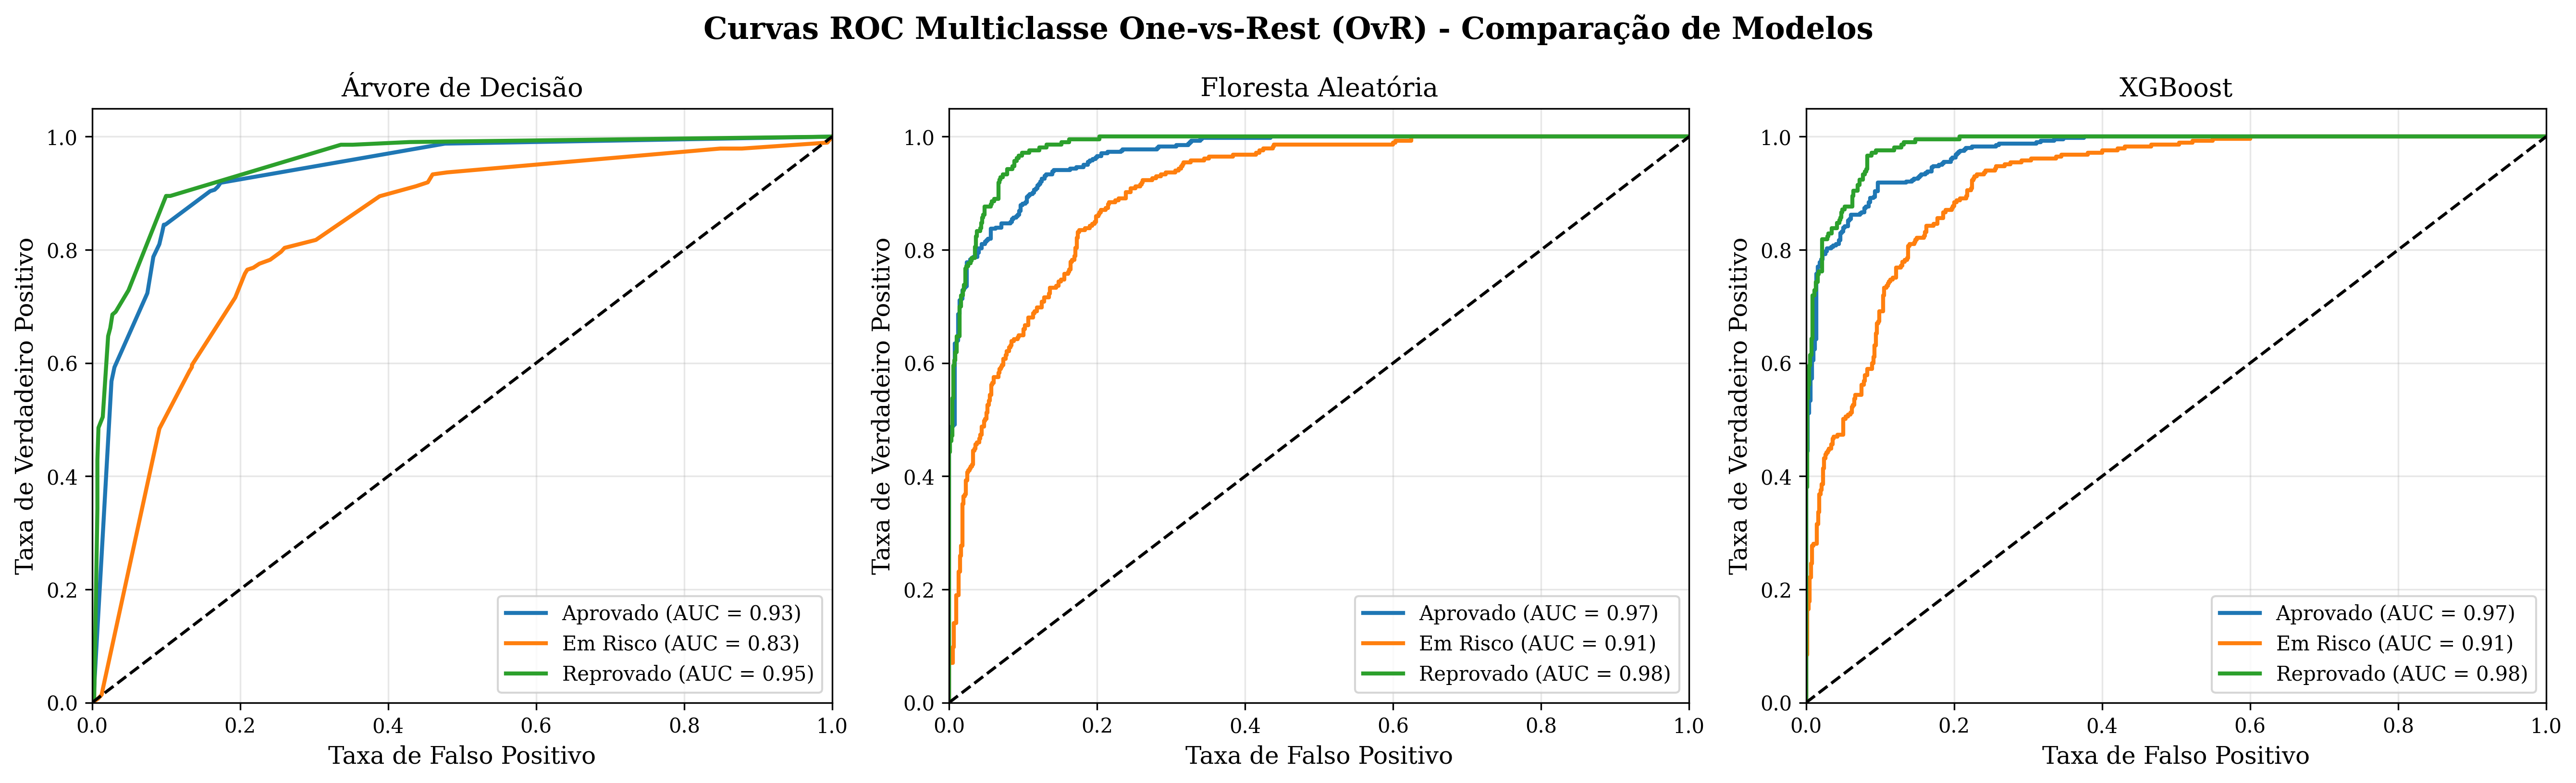
\includegraphics[width=0.98\textwidth]{imagens/roc_curves_comparison.png}
\source{Elaborado pelo autor (2026).}
\end{figure}

No XGBoost, as classes extremas apresentaram excelente separabilidade (AUC de 0,971 para \textit{Aprovado} e 0,983 para \textit{Reprovado}), enquanto a classe intermediária \textit{Em Risco} registrou AUC de 0,915. O mesmo padrão repete-se nos demais modelos (\textit{Decision Tree}: 0,932 / 0,827 / 0,951; \textit{Random Forest}: 0,968 / 0,905 / 0,981, na ordem Aprovado / Em Risco / Reprovado). A menor separabilidade da classe intermediária é esperada e estruturalmente explicável: ela ocupa a banda de fronteira da rotulagem, comprimida por duas fronteiras de decisão simultâneas, e os estudantes próximos aos limiares da LDB compartilham perfis observáveis com as classes vizinhas. Do ponto de vista pedagógico, o desempenho elevado na classe \textit{Reprovado} (\textit{recall} de 84,3\% no XGBoost, com precisão de 87,6\%) é o resultado mais relevante: o modelo raramente deixa de sinalizar o estudante em vulnerabilidade acadêmica severa, minimizando os falsos negativos que mais comprometeriam intervenções preventivas.

\section{Estudo Detalhado das Classes via Matriz de Confusão}

Para investigar a origem granular dos erros de predição, elaborou-se o mapa de calor das matrizes de confusão (Figura~\ref{fig:confusion_comparison}).

\begin{figure}[htb]
\centering
\caption{Matrizes de confusão obtidas nos ensaios de \textit{holdout} (teste).}
\label{fig:confusion_comparison}
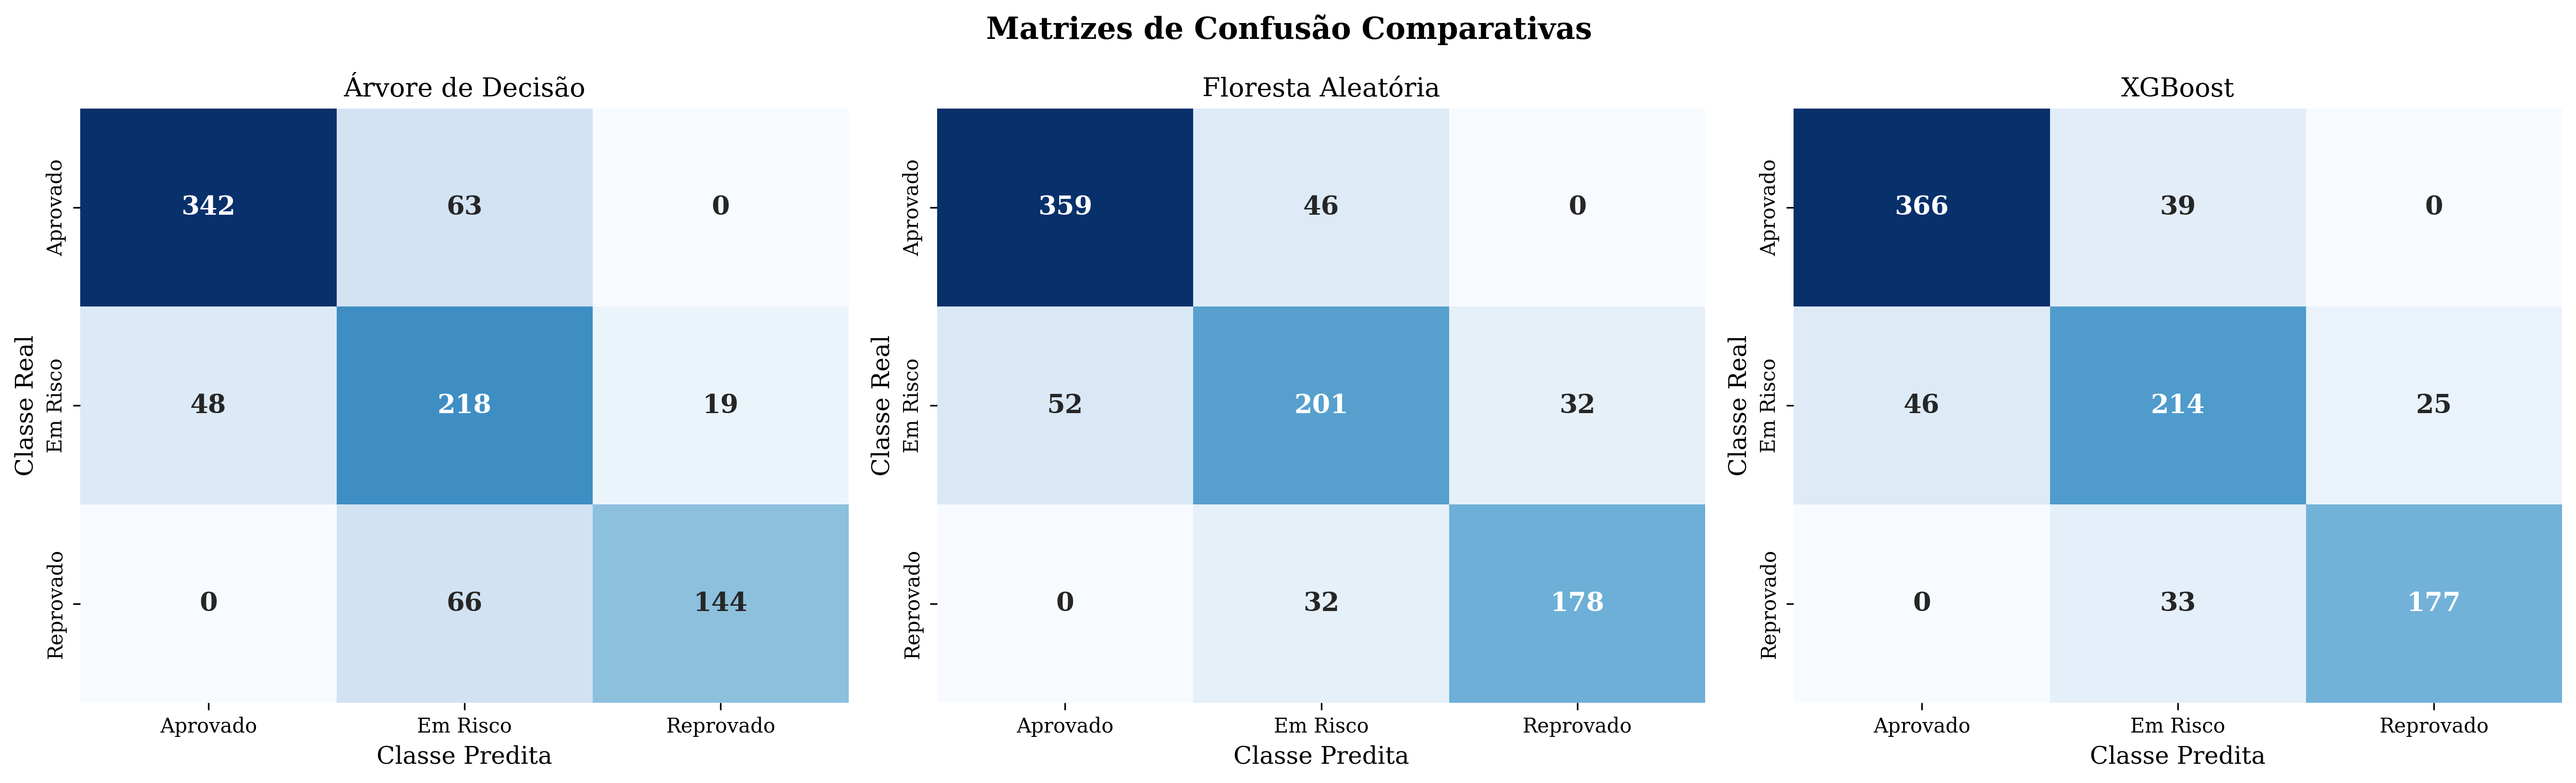
\includegraphics[width=0.98\textwidth]{imagens/confusion_matrices_comparison.png}
\source{Elaborado pelo autor (2026).}
\end{figure}

O achado mais significativo é a \textbf{ausência total de erros entre classes extremas} nos três modelos: nenhum estudante \textit{Aprovado} foi classificado como \textit{Reprovado}, nem o inverso. Todos os erros concentram-se em adjacências ordinais (\textit{Aprovado} $\leftrightarrow$ \textit{Em Risco} e \textit{Em Risco} $\leftrightarrow$ \textit{Reprovado}), o que indica que os classificadores capturaram a ordinalidade latente da tendência de desempenho. No XGBoost, dos 143 erros cometidos em 900 instâncias de teste, 85 ocorreram na fronteira \textit{Aprovado}--\textit{Em Risco} e 58 na fronteira \textit{Em Risco}--\textit{Reprovado} (erros de gravidade operacional reduzida, pois deslocam o estudante para uma categoria vizinha de atenção, sem inverter o prognóstico).

\section{Análise Dimensional e Importância dos Atributos}

A sustentabilidade ética e científica de intervenções educacionais assistidas por aprendizado de máquina exige interpretabilidade. A Figura~\ref{fig:feature_importance} apresenta as contribuições relativas dos atributos em cada classificador.

\begin{figure}[htb]
\centering
\caption{Critério de importância relativa dos atributos na predição de desempenho.}
\label{fig:feature_importance}
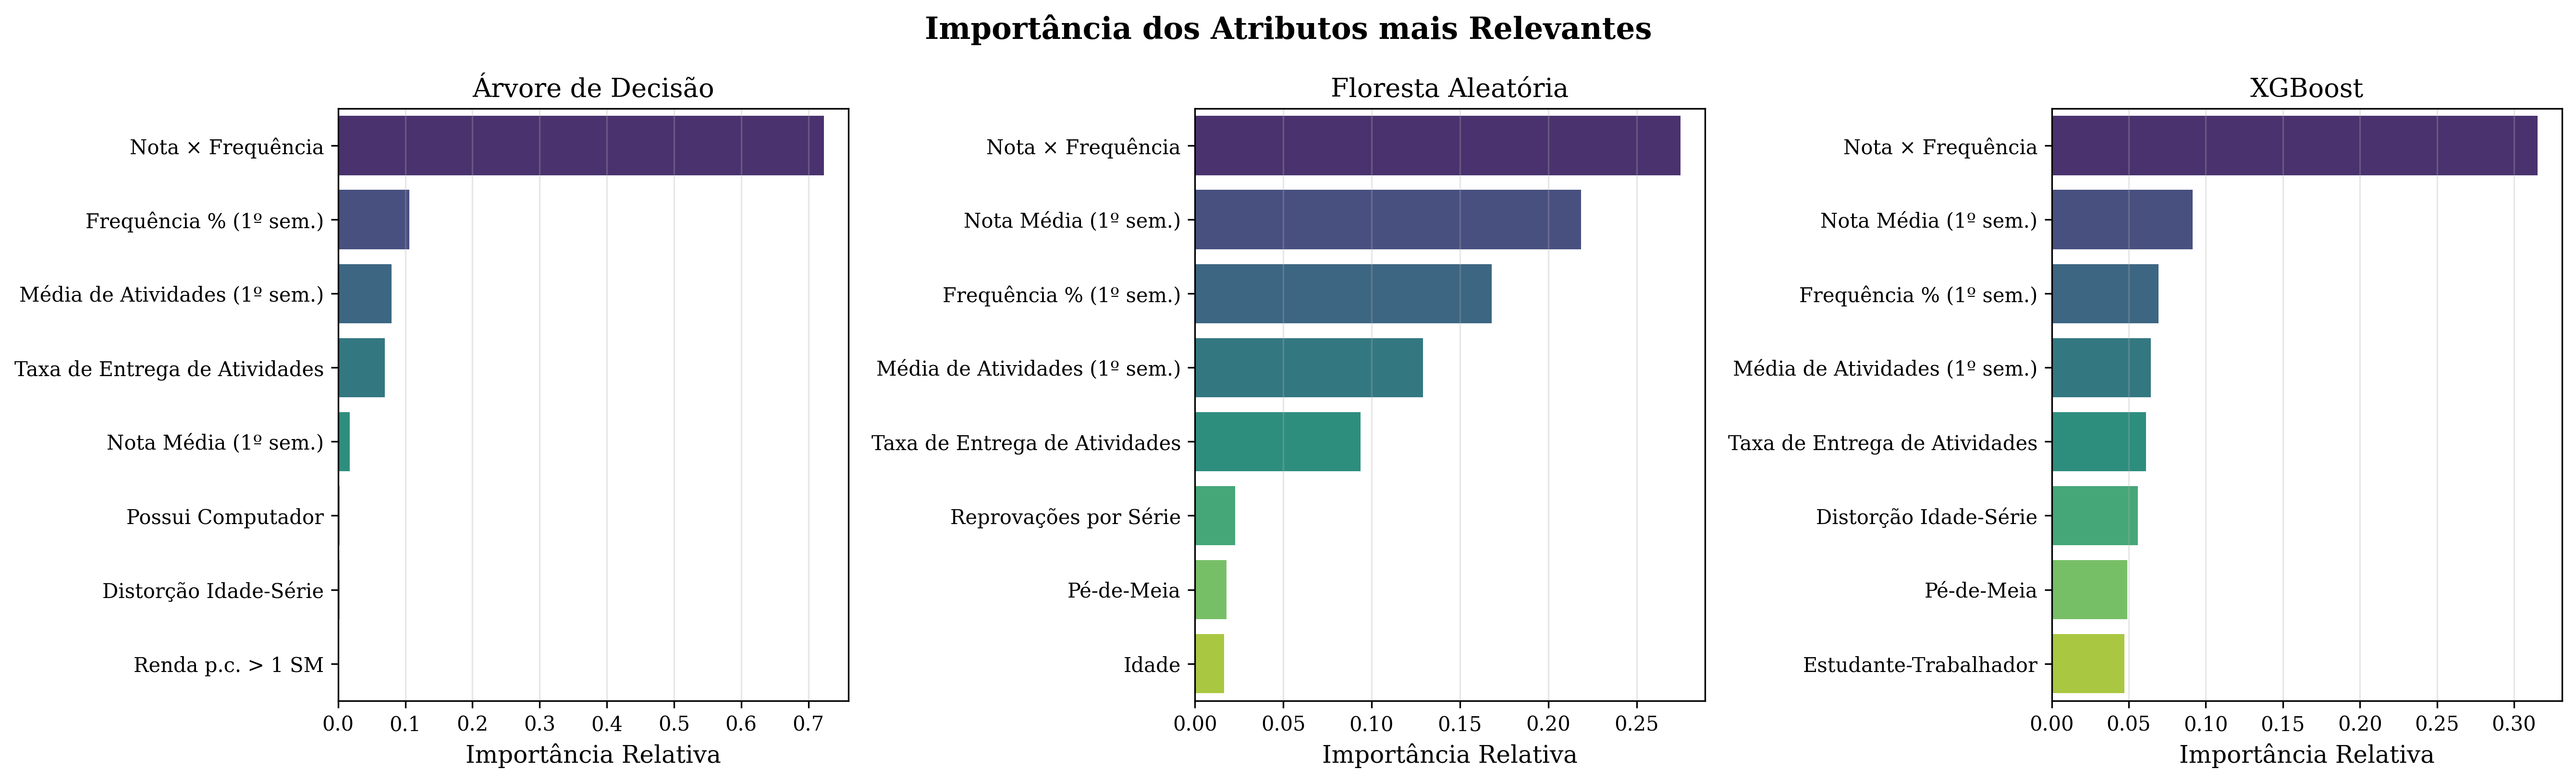
\includegraphics[width=0.98\textwidth]{imagens/feature_importances_comparison.png}
\source{Elaborado pelo autor (2026).}
\end{figure}

A variável derivada de interação nota--frequência (\texttt{nota\_x\_frequencia}) consolidou-se como o preditor de maior relevância em todas as estruturas (cerca de 72\% na \textit{Decision Tree}, 28\% na \textit{Random Forest} e 32\% no XGBoost), corroborando a literatura educacional: nota e frequência não operam isoladamente, mas de maneira sinérgica na representação do rendimento discente \cite{curi2006}. Na sequência aparecem os demais sinais acadêmicos parciais, incluindo as variáveis de engajamento contínuo introduzidas neste trabalho: no XGBoost, a média das atividades responde por 6,4\% e a taxa de entrega por 6,1\% da importância (evidência de que a regularidade do engajamento agrega informação além da nota média e da frequência, em linha com a literatura de EDM \cite{costa2012, fredricks2004}).

O resultado central para a questão de pesquisa, contudo, está na camada seguinte de importâncias do XGBoost: os \textbf{fatores sociológicos} dominam as posições subsequentes: distorção idade-série (5,6\%), recebimento do Pé-de-Meia (4,9\%), trabalho juvenil (4,7\%), renda \textit{per capita} de até meio salário mínimo (3,5\%) e acesso à internet (3,1\%). Cumpre interpretar esse achado nos seus devidos termos: como o fenômeno gerador é sintético, ele não constitui evidência empírica independente de que tais fatores condicionam o desempenho real (essa relação é premissa do gerador, fundamentada na literatura sociológica \cite{berlato2020, marturano2015}). O que o resultado demonstra é de natureza \textbf{metodológica}: os classificadores foram capazes de \textit{recuperar}, a partir exclusivamente dos atributos observáveis, o peso não redundante que os fatores sociológicos receberam no fenômeno gerador, mesmo na presença de indicadores acadêmicos diretos, o que confirma a hipótese H2 e valida a capacidade da arquitetura de capturar essa estrutura quando ela existir nos dados. A posição de destaque do indicador de assistência financeira, em particular, mostra que o modelo capturou o efeito de reversão de tendência do Pé-de-Meia embutido nas regras de geração, cuja fundamentação está na literatura \cite{santos2026}.

Por fim, ressalta-se a salvaguarda anti-viés: gênero e cor/raça foram gerados com peso zero no fenômeno e excluídos do treinamento, juntamente com a origem escolar, de modo que nenhuma decisão do modelo se apoia em atributos demográficos protegidos, uma decisão alinhada às boas práticas de equidade algorítmica em contextos educacionais. As limitações que condicionam a leitura desses resultados são discutidas, em conjunto com suas implicações, na seção de Limitações e Implicações das Considerações Finais.

% ----------------------------------------------------------
% Considerações Finais
% ----------------------------------------------------------
\chapter{Considerações Finais}

O presente trabalho propôs o desenvolvimento de um modelo preditivo de tendência de desempenho acadêmico para estudantes do ensino médio da rede pública estadual do Piauí, fundamentado em fatores sociológicos. Para tanto, foram realizadas duas entregas articuladas: a construção de um conjunto de dados sintéticos com parametrização rastreável a estatísticas oficiais e à literatura acadêmica (no qual os preditores representam sinais parciais do primeiro semestre e o alvo, rotulado pelos critérios de aprovação da LDB, representa a tendência ao final do ano letivo), e a comparação sistemática de três algoritmos de classificação (\textit{Decision Tree}, \textit{Random Forest} e XGBoost) frente a \textit{baselines} de referência, sob o processo KDD, com validação cruzada estratificada ($k=10$), balanceamento por SMOTE confinado a cada \textit{fold} e teste estatístico pareado entre os modelos.

Retomam-se, a seguir, as hipóteses formuladas na Introdução:

\begin{description}
    \item[H1 (confirmada parcialmente).] Os classificadores de \textit{ensemble} superaram a árvore única e os \textit{baselines} com significância estatística (Wilcoxon pareado, $p = 0{,}002$ em ambas as comparações): a \textit{Decision Tree} atingiu 78,22\% de acurácia no \textit{holdout}, a \textit{Random Forest} 82,00\% e o XGBoost 84,11\%, contra 45,00\% do \textit{baseline} majoritário e 80,22\% da Regressão Logística. Entre os dois \textit{ensembles}, contudo, a diferença não é estatisticamente significativa ($p = 0{,}232$): o XGBoost foi adotado como modelo final por sua vantagem numérica consistente, registrando-se a equivalência estatística com a \textit{Random Forest}.
    \item[H2 (confirmada).] Os fatores sociológicos parametrizados no fenômeno gerador foram recuperados pelos modelos como atributos de importância não redundante: após os sinais acadêmicos parciais, as variáveis mais determinantes no XGBoost foram a distorção idade-série, o recebimento do Pé-de-Meia, o trabalho juvenil, a renda \textit{per capita} e o acesso à internet, o que serve como validação metodológica de que a arquitetura captura essa estrutura quando presente nos dados.
    \item[H3 (confirmada).] Os sinais parciais do primeiro semestre foram suficientes para prever a tendência do desfecho anual com desempenho cerca de 39 pontos percentuais acima do \textit{baseline} majoritário, em um cenário com deriva sistemática e idiossincrática de segundo semestre.
    \item[H4 (confirmada).] A regra legal de elegibilidade da assistência financeira produziu, sem qualquer parâmetro dedicado, proporções coerentes de beneficiários entre os cenários: 47,7\% no cenário base, 57,6\% no perfil de alta vulnerabilidade e 6,5\% no perfil de renda alta.
\end{description}

Nos três modelos, nenhum erro ocorreu entre as classes extremas (\textit{Aprovado} e \textit{Reprovado}): todos os equívocos concentraram-se em adjacências ordinais, e a classe crítica \textit{Reprovado} obteve \textit{recall} de 84,3\% no XGBoost (um desempenho relevante para a finalidade preventiva do modelo), pois minimiza os falsos negativos no grupo que mais demanda intervenção pedagógica, em momento do ano letivo no qual a ação preventiva ainda é possível.

O bom comportamento do XGBoost é coerente com suas características arquiteturais: a otimização por aproximação de Taylor de segunda ordem, que incorpora a curvatura da função de perda via Hessiano, e o termo de regularização explícito que penaliza a complexidade das árvores \cite{chen2016}. Essas propriedades permitem ao algoritmo capturar interações não lineares complexas (como a sinergia entre desempenho acadêmico e contexto socioeconômico) que modelos mais simples não representam adequadamente \cite{friedman2001}, ainda que, neste problema, a \textit{Random Forest} tenha alcançado patamar estatisticamente equivalente.

\section{Contribuições do Trabalho}

A principal contribuição desta pesquisa reside na demonstração de que é possível unir, em uma única investigação, a construção de um conjunto de dados sintéticos sociologicamente fundamentado (com rastreabilidade documentada entre cada parâmetro de geração e sua fonte estatística ou acadêmica, incluindo o nível de desagregação e as notas de \textit{proxy}, exportada automaticamente pelo gerador) e a modelagem preditiva comparativa da tendência de desempenho acadêmico. O gerador incorpora mecanismos anti-deterministas ausentes em abordagens ingênuas de simulação: a assistência financeira é derivada de regra de elegibilidade legal (e não de sorteio), as interações entre vulnerabilidades são não lineares, perfis de resiliência acadêmica impedem que os modelos aprendam um determinismo social absoluto, e a rotulagem deriva dos critérios reais de aprovação da LDB, com proporções de classe emergentes.

Adicionalmente, o trabalho contribui para a consolidação de boas práticas metodológicas em Mineração de Dados Educacionais: prevenção de vazamento de dados por meio do SMOTE aplicado exclusivamente no interior de cada partição da validação cruzada \cite{madugula2026}; adoção do F1-Score ponderado como métrica de otimização em cenário desbalanceado \cite{he2009}; inclusão de \textit{baselines} de referência e verificação estatística das diferenças entre modelos \cite{demsar2006}; seleção de variáveis derivadas validada por estudo de ablação; caracterização explícita do teto de acurácia via análise de sensibilidade ao ruído idiossincrático; e salvaguardas de equidade algorítmica, com exclusão de gênero e cor/raça do treinamento. Todo o procedimento é reprodutível e parametrizável, permitindo a simulação de cenários socioeconômicos contrastantes por simples troca de configuração.

\section{Limitações e Implicações}

Não obstante os resultados promissores, algumas limitações devem ser consideradas. A primeira e mais significativa é a natureza sintética da base (em particular, por se tratar de simulação baseada em regras, e não de dados sintéticos derivados de microdados reais): embora cada distribuição marginal seja ancorada em fontes oficiais auditadas, as relações conjuntas entre variáveis refletem as regras especificadas pelo pesquisador. As métricas reportadas medem, portanto, a capacidade dos classificadores de recuperar um fenômeno cuja estrutura (ainda que sociologicamente fundamentada, auditada quanto às fontes e dotada de componente estocástico irredutível) é conhecida por construção, e o desempenho absoluto não deve ser extrapolado diretamente para populações reais. O fenômeno gerador é conhecido por construção, e a transposição para registros reais de estudantes pode revelar padrões, vieses e relações não capturados pela parametrização. A validação com dados reais constitui etapa imprescindível antes de qualquer aplicação prática dos modelos, e as conclusões sobre a importância dos fatores sociológicos devem ser lidas como validação metodológica, não como evidência empírica independente. Como implicação, o valor da evidência produzida está na validação metodológica da arquitetura de classificação, na caracterização do comportamento comparativo dos algoritmos (incluindo a equivalência estatística entre os \textit{ensembles}) e na demonstração de que a estrutura sociológica parametrizada é recuperável pelos modelos a partir dos atributos observáveis.

A segunda limitação refere-se ao recorte do fenômeno: o modelo prevê a tendência do desfecho anual a partir dos sinais do primeiro semestre, sem capturar a dinâmica temporal mais longa da trajetória escolar (transições entre séries, efeitos cumulativos de reprovações sucessivas, sazonalidade da frequência). A terceira concerne à técnica de balanceamento: a literatura recente aponta que a sobreamostragem sintética introduz riscos de privacidade em dados reais (particularmente ataques de inferência de associação), recomendando, para implantações futuras, técnicas de geração com garantias formais de privacidade diferencial \cite{madugula2026, kostopoulos2026}.

Quanto à suficiência dos parâmetros, o conjunto adotado cobre o recorte declarado (sinais parciais intra-ano, contexto socioeconômico individual e desfecho do mesmo ano) e está ancorado nas fontes oficiais e na literatura. Há, contudo, espaço de refinamento: novos atributos de engajamento e de trajetória, substituição do SMOTE pelo SMOTENC nas colunas binárias, repetição da validação cruzada com múltiplas sementes e, sobretudo, a validação com registros reais. Esses refinamentos não invalidam o recorte atual; delimitam a evolução natural do gerador e do procedimento experimental.

Como desdobramentos futuros da pesquisa, destaca-se sobretudo a validação da arquitetura de classificação com registros reais de estudantes (mediante autorização institucional e ética), direção que dialoga diretamente com os trabalhos do grupo de pesquisa voltados à construção de conjuntos de dados institucionais sobre trajetória acadêmica, bem como a integração do modelo a sistemas de gestão escolar, com alertas precoces às equipes pedagógicas, em sinergia com os sistemas \textit{web} de apoio à gestão educacional desenvolvidos no mesmo grupo. Delineiam-se ainda, como extensões metodológicas, a modelagem ordinal e temporal do desfecho, a incorporação de técnicas de IA explicável (SHAP e LIME) para explicações individualizadas das predições, o uso do gerador parametrizável para simulação de contrafactuais de políticas públicas e a adoção de geração sintética com garantias formais de privacidade diferencial nas etapas que envolverem dados reais \cite{kostopoulos2026}.



%% Finalizações para o PDF
\bookmarksetup{startatroot}

%% Elementos pós-textuais: Referências, Anexos, etc.
\input{estrutura/pos-textual}

\end{document}